% siminos/blog/dailyBlog.tex
% $Author$ $Date$

\chapter{Daily blog}
\label{c-DailyBlog}

\begin{description}

\item[2007-06-13 Predrag: Learned nothing from Armbruster {\em et. al}]
Armbruster {\em et. al} showed that four complex Fourier
modes suffice to exhibit most
of the qualitative features of the dynamics,
for a wide range of system sizes\rf{AGHks89}.

\medskip\noindent{\bf 2009-08-28 Predrag} Evangelos in his thesis and
\HREF{http://ChaosBook.org/projects}
     {Kohler in his ChaosBook.org project}
got nothing of interest out of Armbruster \etal\rf{AGHks89}.

\item[2007-11-28 Predrag: Japanese heresy]
We do not want to refer to wrong papers, but here it is, for
the internal record, so we do not forget not to cite it
(from Physical Review Letters, 16 Sep 2004 request to referee,
which I ignored):

Mitsuhiro Kawasaki and Shin-ichi Sasa,
    ``Statistics of unstable periodic orbits of a chaotic dynamical system
    with a large number of degrees of freedom."

\item[2007-11-28 Predrag: Raves]
Amazon.com reviewers rave about \refref{ITO96};
looks nice, get it.
Check out
 \refrefs{ChePiWa02,Jaco05,Kett95,Hall67}.

A free book (but elementary, not useful):
http://www.sst.ph.ic.ac.uk/people/d.vvedensky/courses.html

\end{description}


\section{2007-05-17 $s_1$, $s_2$, $\tau_x$, $\tau_z$ generate 16 irreps?}

\medskip\noindent{\bf Predrag}
 My main problem is - we are currently using only 4 irreducible reps
of $C_2 \times C_2$ = $D_2$ dihedral group generated by $\tau_x, \tau_z$,
but why not 16 irreps of
the $D_2 \times D_2$ generated by $s_1, s_2, \tau_x, \tau_z$?
They all commute, each one splits the space of reps into 2.
Why stop at $U_S$ subspace?
There should be 16 discrete copies of any
general solution, not just 4.
However, there would still be 4 copies of UB, as UB is within the
fully symmetric irrep $A_1$ od $s_1, s_2$ $D_4$.

\section{2008-05-24 ES: Zeghlache Mandel center manifold}

This is just an attempt to understand the primary bifurcation in
Zeghlache and Mandel\rf{ZeMa85} 5-dimensional flow:
\bea
\dot{x}_1 &=&  \sigma (- x_1 -  \delta x_2 + y_1)
               \continue
\dot{x}_2 &=&  \sigma (\delta x_1   - x_2 + y_2)
               \continue
\dot{y}_1 &=& \rho\,  x_1 - y_1 + \delta y_2 - x_1 z
                                                \label{ZMeqs} \\
\dot{y}_2 &=& \rho\,  x_2 - \delta y_1 - y_2 - x_2 z
               \continue
\dot{z}   &=& x_1 y_1 + x_2 y_2  - \gamma\, z
            \,.\nnu
\eea
Here $\sigma>1,\, \rho>0$.

The equation is equivariant under the action of $\Gamma=SO(2)$ defined by
 \beq
 {D}(\theta)
%  =   \left(\barr{ccc}
%     {\bf R}(\theta) &  0              & 0  \\
%     0               & {\bf R}(\theta) & 0  \\
%     0               &  0              & 1
%     \earr\right)
=   \left(\barr{ccccc}
   \cos\theta  &  \sin\theta & 0  &  0 & 0  \\
  -\sin\theta  &  \cos\theta & 0  &  0 & 0 \\
   0  &  0 & \cos\theta  &  \sin\theta & 0  \\
   0  &  0 &-\sin\theta  &  \cos\theta & 0 \\
   0  &  0 & 0  &  0 & 1
   \earr\right)
 \,.
 \label{ZMrotation}
 \eeq

The \stabmat\ is
  \beq
{\Mvar_{ZM}} =
  \left(\barr{ccccc}
    -\sigma    & -\epsilon\sigma & \sigma &  0       &  0 \\
\sigma\epsilon & -\sigma         & 0      & \sigma   &  0 \\
\rho-z         &     0           & -1     & \epsilon & -x_1 \\
0              & \rho-z       & -\epsilon & -1       & -x_2 \\
y_1            & y_2             & x_1    & x_2      & -\gamma
    \earr\right)
\,.
  \ee{ZMstabMat}

The \stabmat\ commutes with ${D}(\theta)$ for points on the
fixed point subspace of $\Gamma$, \ie, the $z$-axis.

The origin is a fixed point of the flow and as it is rotationally invariant (lies on the $z$-axis)
its \stabmat\ has no zero eigenvalue associated with the action of $\Gamma$. For $r<1+\delta^2$
the origin is a stable fixed point, while at $r=1+\delta^2$ the stability
matrix has eigenvalues $ \left(0,0,-\gamma ,-(\sigma+1) \pm i \delta  (\sigma-1) \right)$
and  thus a bifurcation occurs which in the literature\rf{GL-Gil07b} is classified as pitchfork to a
stable circle ($\Gamma$-orbit) of equilibria, while the origin looses stability. This is a surprising
fact because generically \rf{golubII} one would expect an equivariant Hopf bifurcation to a $\Gamma$-invariant periodic
orbit, \ie, a relative equilibrium (traveling wave). Of course, in view of the degenerate zero eigenvalue
of the \stabmat\ at bifurcation we already begin to question the posibility of a Hopf bifurcation.
Nevertheless one should proceed by first reducing the bifurcation problem to one where all of the \stabmat\ eigenvalues
have zero real part, \ie, apply either Lyapunov-Schmidt reduction\rf{golubI} or the Center Manifold Theorem\rf{guckb}.
We follow the latter approach. The procedure is standard but for a five dimensional system I had to use computer algerba
to hope to do it correctly\ES{I only outline the procedure for now, I'll give a better description
and explicit form of transformation matrices, etc, later on if needed.}.

We begin by a linear transformation to new variables $w_i,\, i=1\ldots 5$ such that at bifurcation
the \stabmat\ at the origin is in block-diagonal form. Thus we use the transformation
\beq
	w = T^{-1} x
\eeq
where $w$ and $x$ is shorthand notation for the new and old variables respectively and $T$ is the column matrix of
eigenvectors of \stabmat\ evaluated at the origin, for $\rho=1+\delta^2$. We seek an approximation to the center manifold
as a graph over the center manifold: $w_i = h_i(w_1,w_2,\mu),\, i=3\ldots5$, where $\mu=\rho-1-\delta^2$ is regarded
as the bifurcation parameter but also as an extra variable satisfying $\dot{\mu}=0$. Substituting a Taylor expansion for $h$
up to third order in $w_1,w_2,\mu$ in the transformed equation\ES{actually to a PDE for h which I haven't introduced.} we obtain a local approximation of the center manifold
and we can write the dynamics for $w_1,w_2$ as:
% \begin{eqnarray}
%  \dot{w}_1 & = & \frac{ \sigma}{B^2+F^2}\left[ F\left(\mu +\frac{\left(3 B^2-F^2\right) \mu ^2 \sigma }{\left(B^2+F^2\right)^2}-\frac{w_1^2+w_2^2}{\gamma
%  \left(1+\delta ^2\right)}\right) w_1 + B\left(\mu +\frac{\left(B^2-3 F^2\right) \mu ^2 \sigma }{\left(B^2+F^2\right)^2}-\frac{w_1^2+w_2^2}{\gamma  \left(1+\delta
% ^2\right)}\right) w_2 \right]  \\
%  \dot{w}_2 & = & \frac{ \sigma}{B^2+F^2}\left[ -B\left(\mu +\frac{\left(B^2-3 F^2\right) \mu ^2 \sigma }{\left(B^2+F^2\right)^2}-\frac{w_1^2+w_2^2}{\gamma
%  \left(1+\delta ^2\right)}\right) w_1 + F\left(\mu +\frac{\left(3 B^2- F^2\right) \mu ^2 \sigma }{\left(B^2+F^2\right)^2}-\frac{w_1^2+w_2^2}{\gamma  \left(1+\delta
% ^2\right)}\right) w_2 \right]
% \end{eqnarray}

\begin{eqnarray}
 \left(\begin{array}{c} \dot{w}_1 \\ \dot{w}_2  \end{array}\right) & = & \left[\lambda + g_r(w_1^2+w_2^2) \right]\left(\begin{array}{c} w_1 \\ w_2  \end{array}\right) + \left[\omega + g_\theta(w_1^2+w_2^2) \right] \left(\begin{array}{c} -w_2 \\ w_1 \end{array}\right)
\end{eqnarray}
where
\[\begin{array}{cc}
	\lambda = \frac{ \sigma F}{B^2+F^2} \left(\mu +\frac{\left(3 B^2-F^2\right) \mu ^2 \sigma }{\left(B^2+F^2\right)^2}\right)\,, &
		\omega = -\frac{ \sigma B}{B^2+F^2}\left(\mu +\frac{\left(B^2-3 F^2\right) \mu ^2 \sigma }{\left(B^2+F^2\right)^2}\right) \\
	g_r= -g_\theta= -\frac{ \sigma F}{B^2+F^2} \frac{w_1^2+w_2^2}{\gamma\left(1+\delta ^2\right)}\,,  & B = \delta(\sigma-1)\,,\ F=\sigma+1\,.  \\
\end{array}
\]
In this form it is clear that the reduced system is
$SO(2)$-equivariant and that the eigenvalues of the \stabmat\
vanish at the bifurcation. Thus we can't have a Hopf
bifurcation. On the other hand, for $\mu>0$ and sufficiently
small there is no equilibrium other than the origin, while
there is a $SO(2)$-invariant periodic orbit, \ie, a relative
equilibrium. This is most readily seen if we transform the
system in polar coordinates:
\bea
	\dot{r} &=&\left(\lambda+ g_r(r^2)\right)r \continue
	\dot{\theta} &=& \omega+ g_\theta(r^2)\,.
\eea
This form justifies the use of $g_r,g_\theta$ above. One can see that we cannot have $\dot{r}=\dot{\theta}=0$ for $\mu>0$ and
thus there are no equilibria to the right of the bifurcation point (other than the origin) . On the other hand there exists a Hopf(?) cycle with
\beq
	r^2= \gamma  \left(1+\delta ^2\right) \mu  \left(1+\frac{\left(3 B^2-F^2\right) \mu  \sigma }{\left(B^2+F^2\right)^2}\right)\,,\ \dot{\theta}=\frac{2 B \sigma^2 \mu^2}{\left(B^2+F^2\right)^2}\,,
\eeq
which is a geometrical circle and thus is $SO(2)$-invariant, \ie, it is a relative equilibrium.

This is in direct contradiction with my proof of no existence of relative equilibria in the original system, so something
is wrong. Possibilities are: The application of center manifold theorem was not performed correctly (perharps consider $\delta$
as bifurcation parameter?) One has to go one step further and study the unfolding of the bifurcation (is it codimension-4 bifurcation
or am I counting totally wrong?) I meshed up in proving there aren't relative equilibria in ZM system (did somebody else check at least the polar coordinate representation of the system?) The relative equilibrium in the center manifold is not relative equilibrium in
the original system (sounds crazy but I'll check it.)

{\bf ES} {\refeq{eq:rdcdCLeR} follows from
\cLe\ expressed in the invariant coordinates obtained by the moving frame
method. Since this blog is not explicit transformation
friendly I've added this calculation in my thesis (sec. 4.1.4).
% ({\bf PC:} I fixed the errors in my rewrite - we agree).
We have done the same
for ZM system long time ago when we heuristically
rederived Cartan's method. It has been moved to a footnote in Jonathan's
blog (eq. 5.37) and became one the things that never found their way back to my th
esis.
\\
{\bf PC:} I never understood why ZM system was junked
\\
{\bf ES:} We've agreed to
junk it when we realized it has no \reqva. Also see Sec. 4.1 of my thesis.
One also gets the same system by using invariant
polynomials and taking the syzygy into account, see discussion preceding 5.46 in
Jonathan's blog.
\\
{\bf PC:} please write this up in your thesis - will need it for
the planned publication.}



\section{2008-04-22 ES: Locating Heteroclinic Connections}

I recently tried to locate heteroclinic connections in Lorenz equations. One
can easily see that the 2-dimensional unstable manifold of $\EQV{1}$ intersects the
$2-$dimensional stable manifold of $\EQV{0}$ and thus there should be such connections.
As I couldn't find Predrag's secret method documented somewhere I followed a simple
shooting approach.

Although a heteroclinic orbit is an infinite-time orbit it is sufficient to
pin down a finite time segment of the orbit originating at the linear unstable subspace $E_u^{(1)}$
of $\EQV{1}$ and ending at the linear stable subspace $E_s^{(0)}$ of $\EQV{0}$. Those
requirements can be expressed as the boundary value problem:
\bea
	x(0) & = & \EQV{1}+ \epsilon Re(\mathbf{e}_1^{(1)}) \, \label{eq:shootHetIC} \\
	P_1^{(0)} (x(T)-\EQV{0}) & = &  0 \,. \label{eq:shootHetBC}
%%	P_2^{(0)} (x(T)-\EQV{0}) & = &  d_2 \,. \label{eq:shootHetFixT} %% Not needed for Lorenz
\eea

Eq. \refeq{eq:shootHetIC} imposes the requirement that we start on the unstable subspace of $\EQV{1}$.
Alternatively we could have used as a search space a circle of radius $\epsilon$ on the plane defined
by orthonormalizing $\left(Re(\mathbf{e}_1^{(1)}),\Im(\mathbf{e}_1^{(1)})\right)$, parametrized by some
angle $\theta$. Eq. \refeq{eq:shootHetBC} imposes the condition that the final point on the trajectory is
on the stable manifold of $\EQV{0}$. Here
\beq
	P_j^{(0)}= \prod_{i\neq j}^d \frac{\mathbf{A}(\EQV{0})-\lambda_i^{(0)} \mathbf{1}}{\lambda_j^{(0)}-\lambda_i^{(0)}}\,,
\eeq
is projection operator on the $j$'th eigendirection of the linear stability matrix $\mathbf{A}$ at $\EQV{0}$.
%Condition \refeq{eq:shootHetFixT} needs to be imposed due to the time-translational invariance of the
%equations. It corresponds to restricting the final point on a \Poincare section $\PoincS$ transverse to
%the least contracting eigendirection of $\mathbf{A}(\EQV{0})$. For Lorenz this would be a plane normal
%to the $z$-axis at distance $d_2$ from $\EQV{0}$.
\ES{According to Predrag's notation the left hand side
of equation \refeq{eq:shootHetBC} %%and \refeq{eq:shootHetFixT}
is a scalar.}

To solve the boundary value problem I have used Newton's method to refine a guess for $\epsilon_n$. %and $T_n$
%based on the linearization:
%\beq
%	f^{T_{n+1}}(x_{n+1}) \simeq f^{T_n}(x_n) + \mathbf{J}^{T_n}(x_n) Re(\mathbf{e}_1^{(1)})\delta\epsilon\,, %+ v(f^{T_n}(x_n)) \delta T
%\eeq
%and imposing condition \refeq{eq:shootHetBC} % and \refeq{eq:shootHetFixT}
%on $f^{T_{n+1}}(x_{n+1})$.
Predrag suggests using the linear approximation of the flow to analytically continue the heteroclinic
orbits after period $T$ and impose the condition that this analytic solution ends up on the equilibrium.
I cannot see why this is necessary here. The condition \refeq{eq:shootHetBC} guarantees that the solution
is on the linear approximation of the stable manifold of $\EQV{0}$ and thus will end up on $\EQV{0}$.
Essentially this is the analytic part of the problem and no more needs to be done. The accuracy of the
method is limited by the approximation of the local stable manifold of $\EQV{0}$ and the local unstable
manifold of $\EQV{1}$ by the corresponding linear unstable subspaces, \ie, by planes in the case of Lorenz
equations. One can estimate the distance of minimum approach to $\EQV{0}$ by using the expressions for
the linearized flow. Disregarding the strongly contracting eigendirection $e_3^{(0)}$ I find:
\beq
	r_{min}^2= d_2^2\left(1-\frac{\lambda_2}{\lambda_1}\right)\left(\-\frac{d_1^2 \lambda_1}{d_2^2\lambda_2}\right)^{-\frac{\lambda_2}{\lambda_1-\lambda_2}}
\eeq
where $d_1=P_1^{(0)} (x(T)-\EQV{0})$ and $d_2=P_2^{(0)} (x(T)-\EQV{0})$ \ES{Predrag might want to compare
this against his secret notes.}. I use this to compare with the actual minimum distance from $\EQV{0}$ and
evaluate the validity of the linear approximation of the stable manifold.

In \refref{FriedmanDoedelConnections91} the authors present a
method for computation and continuation of heteroclinic
connections similar in spirit but in a more general setting.
They suggest that a condition breaking the time-translational
invariance should be used along with \refeq{eq:shootHetBC}.
Here, \refeq{eq:shootHetIC} is formulated in a way that
excludes variation in the initial conditions in the direction
of the flow and we need not impose an extra condition.

It works well for Lorenz equations but fails to converge for ZM.



\section{2008-01-17 How to quotient the SO(2) symmetry}
% \section{Symmetry-Reduced Representation (SRR) for KSE}

\medskip\noindent{\bf Ruslan}
In order to quotient the SO(2) symmetry we need to be able to define,
for any state of the KS system $u(x)$
($a = (a_1, a_2, \ldots)^\mathsf{T}$ in Fourier space),
a 'shift' parameter, $s(a) \in S^1 $, such that
\[ \tau_{-s(a)} a \in M/\mathrm{SO}(2). \]
This parameter must satisfy the following {\em monotonicity condition} with
respect to the translation of the state $a$:
\[ s(\tau_{\shift/L}a) = s(a) + \phi(\shift/L) \]
where $\phi(x): S^1 \mapsto S^1$ should be a continuous strictly monotonic function.
This condition is necessary to avoid any ambiguity in the definition of
the shift parameter.

This condition is clearly satisfied when $s(a)$ is proportional to
the first Fourier mode (provided that $|a_1| > 0$)
\begin{equation}
  s(a) =  \theta_1/(2\pi) = \arg(\hat{e}_1^\dagger\,a)/(2\pi)
\label{eq:shift1} \end{equation}
where $\hat{e}_1 = (1+0i, 0, 0, \ldots)^\mathsf{T}$ is the basis vector corresponding
to the first Fourier mode and $\dagger$ denotes Hermitian transpose.
In this case
\[ \arg (e_1^\dagger\,\tau_{\shift/L}a)/(2\pi) = \theta_1/(2\pi) + \shift/L\,, \]
and so $\phi(x) = x$.

It is also possible to get a well-defined shift parameter by
using the difference between phases of Fourier modes $k$ and $k+1$ (provided
that $|a_k|, |a_{k+1}| > 0$):
\begin{equation}
  s(a) = \arg(\hat{e}_{k+1}^\dagger\,a)/(2\pi) -
  \arg(\hat{e}_{k}^\dagger\,a)/(2\pi)\,.
  \label{eq:shiftk} \end{equation}
Maybe for $L = 22$, where dominant Fourier modes are 2 and 3, it is better to use
this shift parameter with $k = 2$?  This needs to be explored.

Of course, as suggested by Predrag, we can define in a similar
fashion the shift parameter with respect to any other
state (e.g. an equilibrium state $a_q$):
\[ s(a) = \arg(a_q^\dagger\, a)/(2\pi)\,, \]
but this shift cannot be guaranteed to satisfy the
monotonicity condition for all $a$.

Since equilibria E1, E2, and E3 for $L = 22$ have dominant
1st, 2nd, and 3rd Fourier modes, respectively, fixing the modes by
Eqs.~(\ref{eq:shift1}) or (\ref{eq:shiftk}) also fixes the equilibria.


\medskip\noindent{\bf 2008-01-17 Monotonicity?}
\medskip\noindent{\bf Predrag:}
Not sure about need for monotonicity - one needs it for the 1-dimensional
Lie group of time evolution, parameterized by a continuous parameter $t$
which can be conjugated to any other parameter $u = u(t,\ssp)$ as long
as it is monotone, but rotations can go whichever way they want, modulo
$2\pi$ (or $L$). Once we look at a problem with $SO(3)$ symmetry, what's the
need for monotonicity in Euler angles, \etc.?

\medskip\noindent{\bf 2008-01-17 Ruslan I think we need monotonicity.}
Let us say $s(a)$ is defined in such a way that it is not monotonic with respect to
shifts of state $a$.  Then there could exist $\shift_1$ and $\shift_2 \neq \shift_1$ such that
\[ s(\tau_{\shift_1/L}\,a) = s(\tau_{\shift_2/L}\,a) = s\,. \]
Then $\tau_{\shift_1/L - s}\,a$ and $\tau_{\shift_2/L - s}\,a$ would be two distinct points
in $M$/SO(2) representing the same state $a$.  This doesn't seem right.

\section{2009-05-21 Talked to Rowley}

\noindent{\bf Evangelos}
I am working on quotienting KS in a some sense. I am in
Snowbird so I got the chance to talk to a few people about
it. I've talked to Gilmore who initially said he cannot help
us with symmetry reduction in thousands of dimensions
(apparently you've talked to him last fall about it) but came
to my talk and got interested I think, asked for the paper
and/or thesis when available. The talk went well I believe.

I've also talked to Rowley (as in Rowley and Marsden). What
they do for "transverse" integration is somewhat different to
what we do for CLe. Their transverse integration depends on
the reconstruction equation (while for us it is totally
independent) so that if the reconstruction equation fails
(there is a denominator that can vanish in it) the whole
procedure, not just reconstruction, has to be restarted with
different "template". This is what makes their method local.
We don't have such problems I think.

\begin{description}
\item[Predrag]
Rowley is right, see \refsect{sect:epyc2Fourier}.

\item[Evangelos]
Also talked a little bit with Kevin Mitchel about the
geometrical origin of singularities. He is not against the
modified invariants and I think he is right about the
impossibility of global reduction with purely geometrical
means.
\end{description}

\section{2009-08-03 Method of slices for \cLf}
\renewcommand{\ssp}{x}

\begin{description}
\item[2009-08-03 Predrag]
here is some summer work that I had originally inserted into
\\
dasbuch/book/chapter/continuous.tex in fit of over enthusiasm
- because Evangelos praised it: ``It works like charm.''
Unfortunately, it did not - the slice described here suffers
from the usual discontinuities.


\item[\Slice\ for \cLf.]
%from \Chapter{continuous}{26sep2009}{Relativity for cyclists}
Here we can use the fact that
\[ \groupTan(\sspRed) \cdot \sliceTan{}
 = \sspRed \cdot \Lg^T \,\Lg \, \slicep
 =
    \bar{x}_1 x_1'
   +\bar{x}_2 x_2'
   +\bar{y}_1 y_1'
   +\bar{y}_2 y_2'
\]
is the dot-product restricted to the 4-dimensional
representation of $\SOn{2}$.
A generic  $ \slicep $ can be brought to form $ \slicep  =
(0,1,y_1',y_2',z)$ by a rotation and rescaling. Then $\Lg
\cdot \slicep   = (1,0,y_2',-y_1',0)$, and
%                                                        \exerbox{exer:csectionReduced}
\beq
\frac{\vel \cdot \sliceTan{}}{\groupTan(\sspRed) \cdot \sliceTan{}}
= -
\frac{\vel_1 + \vel_3 y'_2 -\vel_4 y'_1}
     {\bar{x}_2 + \bar{y}_1 y'_1 + \bar{y}_2 y'_2}
%\frac{\vel_1 x'_2 -\vel_2 x'_1 + \vel_3 y'_2 -\vel_4 y'_1}
%     {\vel_1 x'_1 + \vel_2 x'_2 + \vel_3 y'_1 + \vel_4 y'_2}
\,.
\label{PCsectSin}
\eeq
%%%%%%%%%%%%%%%%%%%%%%%%%%%%%%%%%%%%%%%%%%%%%%%%%%
% computed by wilczak/matmematica/PCsection.nb
\SFIG{PCunrot3}
{}{
Method of moving frames, \slice\ fixed by a point on the \cLe\
\reqv\ group orbit, $\slicep  = \ssp_{\REQV{}{}1}$. The strange
attractor of \cLf\
%\reffig{fig:CLEx1x2z}
in the \reducedsp, %\ of \refeq{EqMotionMovFramePC}
, $\{x_1,x_2,z\}$.
}
{fig:PCunrot3}
%%%%%%%%%%%%%%%%%%%%%%%%%%%%%%%%%%%%%%%%%%%%%%%%%%
%
A long time trajectory of \cLf\ %\refeq{EqMotionMovFramePC} with
$\slicep$ on the \reqv\ \REQV{}{1} group orbit is shown in
\reffig{fig:PCunrot3}.
As initial condition
we chose an initial point % \refeq{eq:REQB1velocVal}
on the unstable manifold
of \REQV{}{1}, rotated back to the \slice\ by angle $\gSpace$.
% as prescribed by \refeq{PCsectQ1}.
In \reffig{fig:PCunrot3} we
show the part of the trajectory for $t\in\left[70,100\right]$.
The \reqv\ \REQV{}{1}, now an equilibrium of the
\reducedsp\ dynamics, organizes the flow into a R\"ossler type
attractor.
% (see \reffig{RosslerAtractor}).
There appears to be no singularity in this
projection although we can run into trouble % with \refeq{EqMotionMovFramePC}
wherever the denominator in $\dot{\theta}$ % \refeq{MFdtheta}
vanishes, \ie, the direction of group
action on the point $\ssp$ is perpendicular to the direction
of group action on $\slicep$.
%                                                        \exerbox{exer:PCsectionCLe}
    \PC{
Apparent lack of singularities in \reffig{fig:PCunrot3} appears
fortuitous.
Diverging velocities subspace is a 4\dmn\ subspace, and indeed our simulations encounter
this subspace very quickly, with \reducedsp\ velocity going off to infinity.
    }

%%%%%%%%%%%%%%%%%%%%%%%%%%%%%%%%%%%%%%%%%%%%%%%%%%
% computed by wilczak/matmematica/PCsection.nb
\SFIG{PCunrot2}
{}{
Method of moving frames, \slice\ as in \reffig{fig:PCunrot3},
but $\{x_2,y_2,z\}$ projection. The \cLf\ strange attractor
% of \reffig{fig:CLEx1x2z}
now exhibits a discontinuity due to
vanishing denominator in \refeq{PCsectSin}.
}
{fig:PCunrot2}
%%%%%%%%%%%%%%%%%%%%%%%%%%%%%%%%%%%%%%%%%%%%%%%%%%

Indeed, the method does encounter singularities in
subsets of \statesp, with phase velocity $\dot{\gSpace}$
divergent whenever the denominator in \refeq{PCsectSin}
changes sign, see \reffig{fig:PCunrot2}.
Hence a single \slice\ does
not in general suffice to cover $\pS/\Group$ globally.

%From dasbuch/book/chapter/continuous.tex \section*{Flotsam}
%
The moving frames method allows the determination of (non-polynomial)
invariants of the group action by a simple and efficient
algorithm that works well in high-dimensional \statesp s.
    \PC{Evangelos, add references here? {\bf ES}: mmm... SiminosThesis?}
    \PC{Evangelos, why ``(non-polynomial)'' invariants?
        length$^2$ is polynomial {\bf ES}: It is the only one though.
        {\bf PC}: is this an answer?}

%
%%%%%%%%%%%%%%%%%%%%%%%%%%%%%%%%%%%%%%%%%%%%%%%%%%%%%%%%%%%%%%%%%%
% CLEpcSect.png computed by  CLEfinal.nb (repo: vaggelis)
% CLEpcSect2.png computed by CLEfinal.nb (repo: vaggelis)
% Predrag's program: wilczak/matmematica/PCsection.nb
\begin{figure}[ht]
\begin{center}
(a) 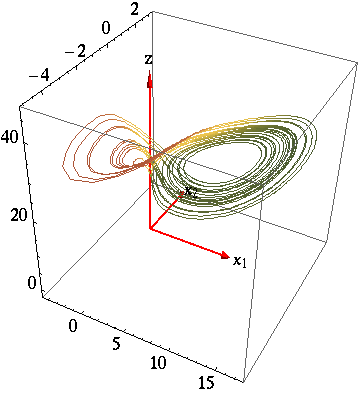
\includegraphics[width=0.40\textwidth]{CLEpcSect}
(b) 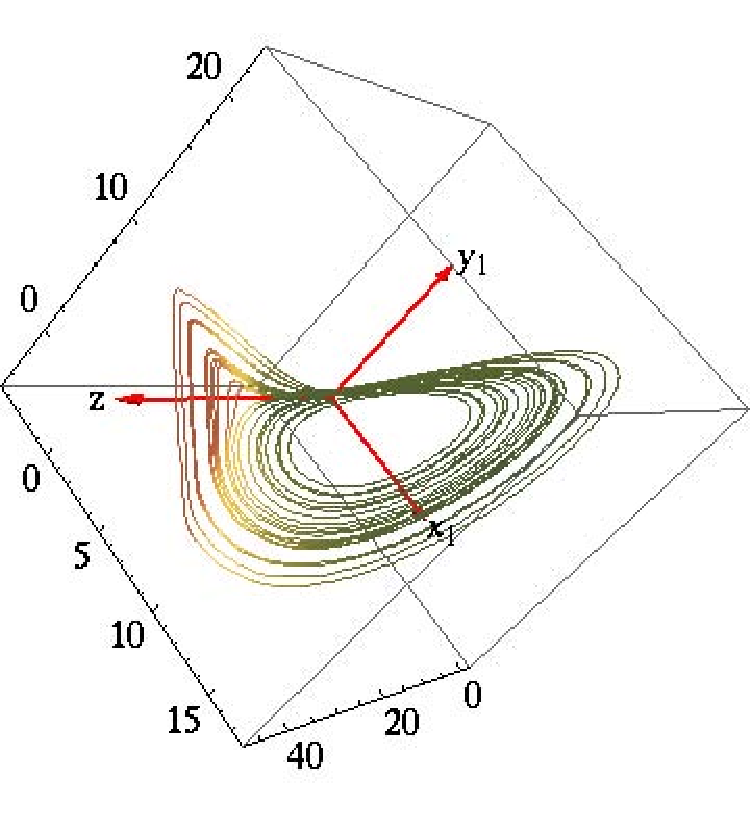
\includegraphics[width=0.43\textwidth]{CLEpcSect2}
\end{center}
\caption{
Method of moving frames, \slice\ fixed by a point on the \cLe\
\reqv\ group orbit, $\slicep  = \ssp_{\REQV{}{}1}$. The strange
attractor of \cLf\ %\reffig{fig:CLEx1x2z}
in the \reducedsp:
% of \refeq{EqMotionMovFramePC}:
(a) $\{x_1,x_2,z\}$ projection,
(b) $\{x_1,y_1,z\}$ projection.
Color-coding indicates $(\hat{\ssp} \cdot \hat{\slicep })_4$
where $\hat{.}$ stands for unit vector, with green indicating values
of the inner product close to $1$ and brown indicating values
close to $0$.
% \authorES
    }
\label{fig:CLEpcSect}
\end{figure}
%%%%%%%%%%%%%%%%%%%%%%%%%%%%%%%%%%%%%%%%%%%%%%%%%%%%%%%%%%%%%%%%
%
    \ES{I will add a scale in \reffig{fig:CLEpcSect} but it is too
   late here to do it tonight.}
    \PC{will need quality CLEpcSect.eps, CLEpcSect2.eps}
    \PC{ in \reffig{fig:CLEpcSect}:\\
        * Mark $\ssp_{\REQV{}{}1}$ \\
        * Draw stable eigenvector of $\ssp_{\REQV{}{}1}$\\
        * State value of $\ssp_{\REQV{}{}1}$ somewhere
        }
%
%%%%%%%%%%%%%%%%%%%%%%%%%%%%%%%%%%%%%%%%%%%%%%%%%%
% computed by PCunrot.nb
\SFIG{PCunrot1}
{}{
Method of moving frames, continuous time version, for the
polar coordinates motivated $x'=(0,1,0,0,z)$,
$x_1=0,\;x_2>0$, \slice. The \cLf\ strange attractor of \cLf\
% \reffig{fig:CLEx1x2z}
exhibits a discontinuity at
$x_2=0$ in the \reducedsp:
$\{x_2,y_2,z\}$ projection.
}
{fig:PCunrot1}
%%%%%%%%%%%%%%%%%%%%%%%%%%%%%%%%%%%%%%%%%%%%%%%%%%
%
Indeed, the method does encounter singularities in
subsets of \statesp.
For example, the \reducedsp\ equations \refeq{PCsectSin}
for the polar coordinates inspired \slice\
$x'=(0,1,0,0,z)$, $x_1=0,\;x_2>0$,
%this is illustrated by \reffig{fig:PCunrot}.
%$(\rho_1,\gSpace_1)$ are polar coordinates, $\rho_1 =
%\sqrt{\ssp_1^{ 2} + \ssp_2^{2}}$, see \refeq{eq:CartToPol},
are given by
%                                                    \exerbox{exer:csectionCLe}
\beq
\dot{\ssp} = \vel - \frac{\vel_1}{\sspRed_2} \, \sliceTan{}
\,,
\ee{EqMotionMovFrame1}
with phase velocity $\dot{\gSpace}$ divergent whenever $\sspRed_2$
changes sign, see \reffig{fig:PCunrot1}.

\item[Predrag's `method of connections']

%
%%%%%%%%%%%%%%%%%%%%%%%%%%%%%%%%%%%%%%%%%%%%%%%%%%
% from Rowley-Marsden paper
\SFIG{connections}
{}{
Method of connections, as illustrated by Rowley and
Marsden\rf{rowley_reduction_2003}.
}
{fig:connections}
%%%%%%%%%%%%%%%%%%%%%%%%%%%%%%%%%%%%%%%%%%%%%%%%%%
%


We decompose $\vel(x)$
in a part $\vel_\shortparallel$ parallel
to the group action and a part $\vel_\perp$ transverse to it,
\beq
	\vel(\ssp)=\vel_\shortparallel(\ssp)+\vel_\perp(\ssp)\,,
\ee{flowSplit}
using the projection operator
\beq
 	?? %\PperpOp_{ij}(\ssp)
 =\delta_{ij}-
    \frac{ \groupTan(\ssp)_i \groupTan(\ssp)_j}{\groupTan(\ssp)^2}
\ee{transvProj}
that projects a $d$-dimensional flow $v(\ssp)$ onto
flow
\beq
	\dot{\ssp}_\perp = \vel_\perp(\ssp) = \vel(\ssp)
    - \frac{\groupTan(\ssp) \cdot \vel(\ssp)}{\groupTan(\ssp)^2}
      \, \groupTan(\ssp)
\ee{transvFlow}
in a $(d\!-\!1)$-dimensional {\csection} transverse to the
direction fixed by the point $\ssp$. By ignoring the flow
component that can be compensated for by an $\SOn{2}$
rotation we quotient the flow by $\SOn{2}$.

For an illustration, Rowley and
Marsden\rf{rowley_reduction_2003} \reffig{fig:connections}.


Note, however, that a choice of $\ssp_0$ fixes only a
direction, so the reduced flow is still equivariant under the
action of discrete cyclic group $\Ztwo = \{e,D(\pi)\}$ on
$\ssp$, $\vel(\ssp)$ and the reference point $\ssp_0$, just
as was the case %\refeq{LorenzR}
for the Lorenz flow. %\refeq{Lorenz}.
    \PC{\emph{Mea culpa}: Here I screwed up. I forgot that rotation
    moves $\vel$ and counter-moves $\ssp$ in $\vel(\ssp)$, \ie,
    acts by the Lie derivative \refeq{inftmInv}. I could never
    understand why we do not see a translational zero eigenvalue
    everywhere (the Lie group acts globally and commutatively
    right?), but only on \eqva, \reqva\ and \rpo s. Presumably
    the projection operator \refeq{transvProj} is OK for the
    \reqv\ calculation of \refeq{sect:StabEq},
    as the action of the group on $\ssp_{\REQV{}{1}}$ is trivial?
    Not sure how to rewrite the decomposition induced by
    \refeq{transvProj} correctly, in
    terms of the full Lie derivative action, and not only the $\Lg$
    action.
    }


\item[Predrag's integral of the equivariance condition]
Here is a suspect attempt to derive a connection formula.
Integrate the equivariance condition \refeq{inftmInv}:
\bea
{const} &=& (\Lg_a)_{kj}
          \int_0^t d\tau \left(
  \delta_{ik}\vel_j(\ssp) - \Mvar_{ik}(\ssp)\, \ssp_j
           \right)
  \continue
  &=& (\Lg_a)_{ij} (\ssp_j(t)-\ssp_j(0))
    - (\Lg_a)_{kj} \int_0^t d\tau \Mvar_{ik}(\ssp(\tau))\, \ssp_j(\tau)
    \continue
  &=& t(\ssp) - t(\ssp_0) - \int_0^t d\tau \Mvar (\ssp(\tau))\, t(\ssp)
  \,.
\label{integralInv}
\eea
If $const=0$, this is a formula for the transport of the group
tangent field,
\[
t(\ssp) = t(\ssp_0) + \int_0^t d\tau \Mvar (\ssp(\tau)) \, t(\ssp(\tau))
\,,
\]
which is not simply the multiplication by \jacobianM\ $\jMps$.
For a linear flow, this looks a bit unfamiliar:
\[
t(\ssp) = t(\ssp_0) + \Mvar\,\Lg_a \int_0^t d\tau \, \ssp(\tau)
\,.
\]
\end{description}

\section{2009-08-26 Method of slices for an $U(1)$-equivariant linear model}
\renewcommand{\ssp}{a}

%{\em \underline{Preamble:} My gut tells me that the method
%of moving frames, as described in the Section 4.2 of the
%thesis will \underline{not} work for KS.  But since my brain
%is dafter than my gut, I cannot explain why I feel that way.
%So, in order to make progress in this direction, I'm going to
%work with a dynamical system similar to KS, but much simpler.
%If I can figure out how to apply the moving frames to this
%system, then I can do it for KS as well.  If not, then I hope
%it will help me understand why my gut is right. \vspace{2ex}}

\medskip\noindent{\bf Ruslan} Forget \KS, let's consider a simpler dynamical system.
Let us say that, just like KS, we have a dynamical system on the space of real function $u(x,t)$ periodic in $x \in [-\pi, \pi)$, i.e. $u(x+2\pi,t) = u(x,t)$.  In the Fourier space $a = \mathcal{F}[u]$, $a = (a_1, a_2, \ldots)$, $a_k \in \mathbb{C}$ and $a_{-k} = a_k^\ast$.
I will also use polar coordinates, so $a_k = r_k \mathrm{e}^{i \phi_k}$.
The action of $U(1)$ on $u(x,t)$ is $g(\theta) u(x,t) = u(x+\theta,t)$. In the Fourier space
\[ g(\theta) a_k = \mathrm{e}^{ik\theta}a_k\,, \]
%In polar coordinates $\tau_{\shift/L} (r_k, \theta_k) = (r_k, \theta_k + q_k \shift)$.
To define the $U(1)$ group rotation tangent $t(a)$, we consider an infinitesimal rotation
\[ \mathrm{e}^{ik\theta}a_k = (1 + ik\theta)a_k  = a_k + \theta t_k\,, \]
so $t_k = ika_k$.
In matrix notation, $\mathbf{T} = \mathrm{diag}(ik)$,
    so  $t = \mathbf{T}a$.

The equation defining the slice through some point $\slicep$ is
\[ (\bar{a} - \sliceTan{}) \cdot \sliceTan{} = 0 \]
By the dot product we mean
\[ a \cdot b = \sum_{k=-\infty}^\infty a_k b_k^*\,, \]
which in the space of real periodic functions corresponds to
\[ f \cdot g = \int_{-\pi}^\pi f(x) g(x) dx\,, \]
where $f(x) = \mathcal{F}^{-1}[a]$ and $g(x) = \mathcal{F}^{-1}[b]$,
so this makes sense.  But note that this is not
the only way of defining the dot product.

\subsection{2009-08-26 Epicycles: 2-Fourier modes}
\label{sect:epyc2Fourier}

\medskip\noindent{\bf Ruslan}
Let us define a 2-Fourier modes linear dynamical system
$\dot{a}_k = v_k(a)$ as follows: $v_k = i \omega_k a_k$,
$\omega_{-k} = -\omega_k$, where $\omega_k \in \mathbb{R}$ are
constants.
    \RLD{$\omega_{-k} = -\omega_k$.
    I used this in my derivation to get the sign right.
    {\bf Predrag} Agreed - I used that too in rederiving your model.}
This
\HREF{http://www.c2.com/cgi/wiki?AddingEpicycles}
     {``epicycles'' model}
is a linear dynamical system, so we can solve it analytically:
\[ a_k(t) = a_k(0) \mathrm{e}^{i \omega_k t} \]
Even simpler, I'm going to use only the first two modes, so $a_k(0) = 0$ for all $|k| \neq 1$ or 2.

We can choose constants $\omega_1$ and $\omega_2$ such that this system can have
a traveling wave or a RPOs in the original space of periodic functions $u(x,t)$.\\
{\bf Example 1: \Reqv.} If $\omega_1 = c$ and $\omega_2 = 2c$, then
\[ a_k(t) = a_k(0) \mathrm{e}^{ikct} = g(ct) a_k(0)\,, \]
which is a wave traveling with speed $c$.\\
{\bf Example 2: \Rpo.} For the system to have an RPO, we can choose, for example,
$\omega_1 = \pi/2$ and $\omega_2 = 3\pi$.  This RPO has period $T = 1$ and shift $\pi/2$, since
\[ a_1(1) = a_1(0) \mathrm{e}^{i\pi/2} = g(\pi/2) a_1(0) \quad \mathrm{and} \quad
   a_2(1) = a_2(0) \mathrm{e}^{i3\pi} = a_2(0) \mathrm{e}^{i\pi} = g(\pi/2) a_2(0) \]

Let us now see what happens if we apply the method of slices to these two examples.
The reconstruction equation is
\[ \dot{\theta} = \frac{v(\bar{a}) \cdot \sliceTan{}}{t(\bar{a}) \cdot \sliceTan{}} \]
Let us say the initial condition $a_1(0) = r_1 > 0$, $a_2(0) = r_2 > 0$
(i.e. $\phi_1 = \phi_2 = 0$) is also the point $\slicep$ defining the slice.  Then
$\sliceTan{k} = ikr_k$ when $|k| = 1,2$ and zero otherwise.  So,
\beq
\dot{\theta} = \frac{\sum_k (i\omega_k \bar{a}_k) (ikr_k)^*}{\sum_k (i k \bar{a}_k)(ikr_k)^*}
                = \frac{\sum_k k \omega_k \bar{a}_k r_k}{\sum_k k^2 \bar{a}_k r_k}
\ee{RLDrec}
The equation for the flow on the slice (aka reduced flow) is
\beq
\dot{\bar{a}}_k = v_k(\bar{a}) - \frac{v(\bar{a}) \cdot \sliceTan{}}{t(\bar{a}) \cdot \sliceTan{}} t(\bar{a})
                   = i\omega_k \bar{a}_k - \frac{\sum_k k \omega_k \bar{a}_k r_k}{\sum_k k^2 \bar{a}_k r_k} ik\bar{a}_k\,.
\ee{RLDred}
\medskip\noindent{\bf Predrag}
I have coded \texttt{wilczak/matematica/PCruslan.nb} also for
$\slicep$ complex, if we need it - no reason to chose it real,
though experimentally it seems not to be the cause of the singularity in
$d\theta/dt$.

\noindent {\bf Example 1: \Reqv.} Here $\omega_k = kc$, so we immediately get
\[ \dot{\theta} = c \quad \mathrm{and} \quad \dot{\bar{a}}_k = 0\,, \]
as expected for the traveling wave.\\
{\bf Example 2:  \Rpo.} In general, for the flow with two non-zero
modes (remembering that $a_{-k} = a_k^*$ and $\omega_{-k} =
-\omega_k$):
\beq
 \dot{\theta} = \frac{\omega_1 r_1 (\bar{a}_1 + \bar{a}_1^*)
                  + 2\omega_2 r_2 (\bar{a}_2 + \bar{a}_2^*)
                  }{r_1(\bar{a}_1 + \bar{a}_1^*) + 4r_2 (\bar{a}_2 + \bar{a}_2^*)}
\ee{Period1}
and
\[ \dot{\bar{a}}_k = i\omega_k \bar{a}_k - \frac{\omega_1 r_1 (\bar{a}_1 + \bar{a}_1^*) + 2\omega_2 r_2 (\bar{a}_2 + \bar{a}_2^*)}{r_1(\bar{a}_1 + \bar{a}_1^*) + 4r_2 (\bar{a}_2 + \bar{a}_2^*)}ik\bar{a}_k \]
When $\omega_1 = \pi/2$ and $\omega_2 = 3\pi$, the second equation should generate a periodic orbit with period $T = 1$, while the solution of the first equation, starting with $\theta(0) = 0$, should give us $\theta(1) = \pi/2$.  Unfortunately, we cannot solve these equations analytically, so I'll do it numerically for different values of $r_{1,2}$.  I'll set $r_1 = 1$ and increase $r_2$ from zero.  Note that when $r_2 = 0$, we just have a traveling wave with speed $\omega_1$.  Also, when $r_2$ is sufficiently smaller than $r_1$, we will have a traveling wave slightly modulated by the 2nd mode.  This case is shown in the figure below:

\vspace{2ex}\noindent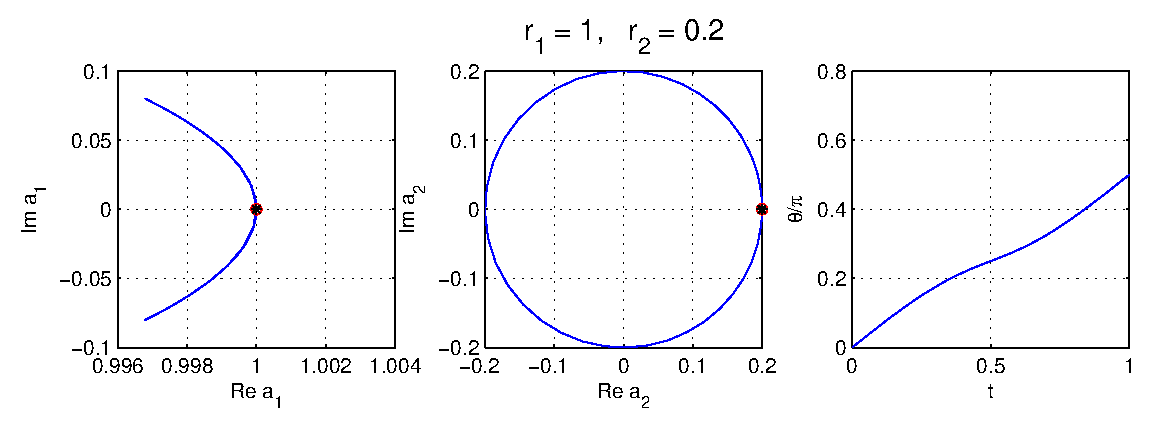
\includegraphics[width=\textwidth]{sliceflow1.eps}

So, everything works well: the reduced orbit is periodic (the beginning of the orbit is denoted by the red circle, while the end is denoted by the black asterisk), and the phase shift at $t = 1$ is equal to $\pi/2$.  We can see similar picture when we increase $r_2$:

\vspace{2ex}\noindent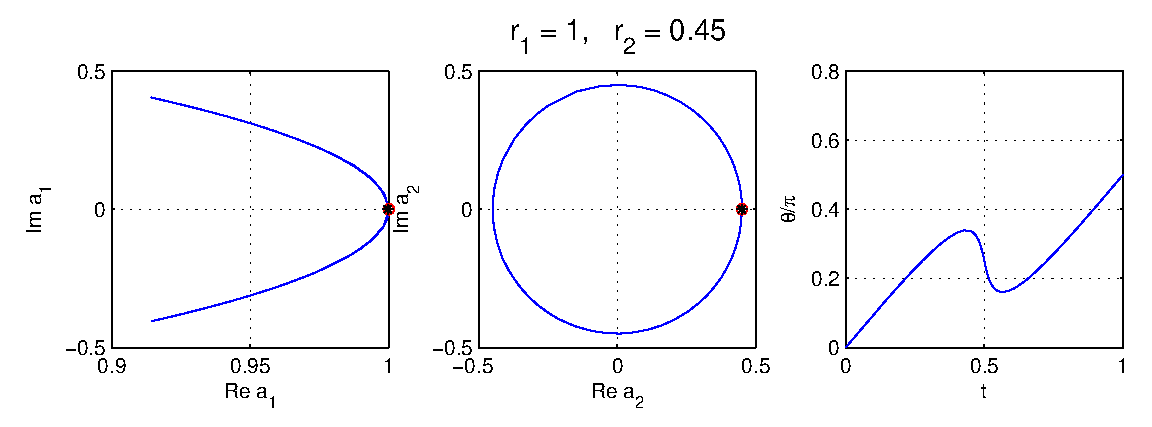
\includegraphics[width=\textwidth]{sliceflow2.eps}

Now, when $r_2$ approaches 0.5, it is clear that the orbit approaches a singularity:

\vspace{2ex}\noindent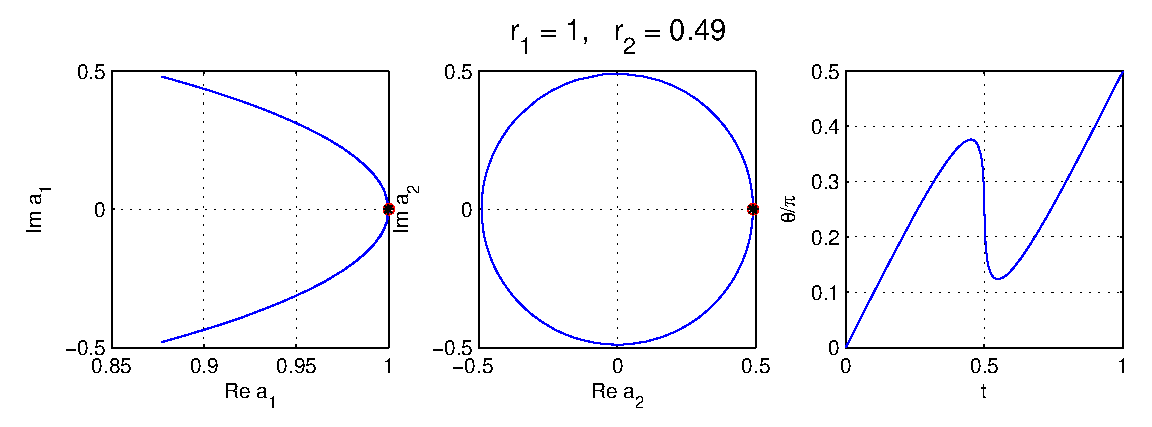
\includegraphics[width=\textwidth]{sliceflow3.eps}

At $r_2 = 0.5$ we get rubbish:

\vspace{2ex}\noindent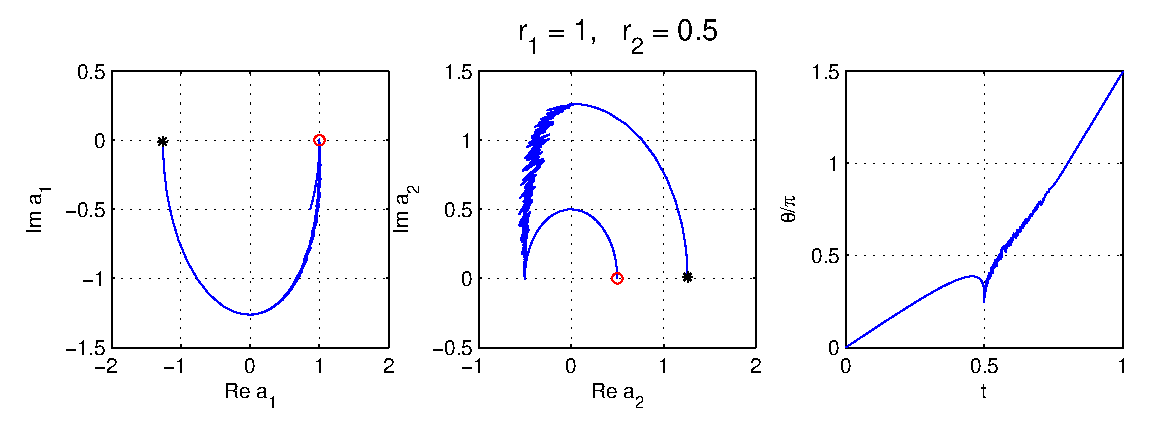
\includegraphics[width=\textwidth]{sliceflow4.eps}

which persists for awhile

\vspace{2ex}\noindent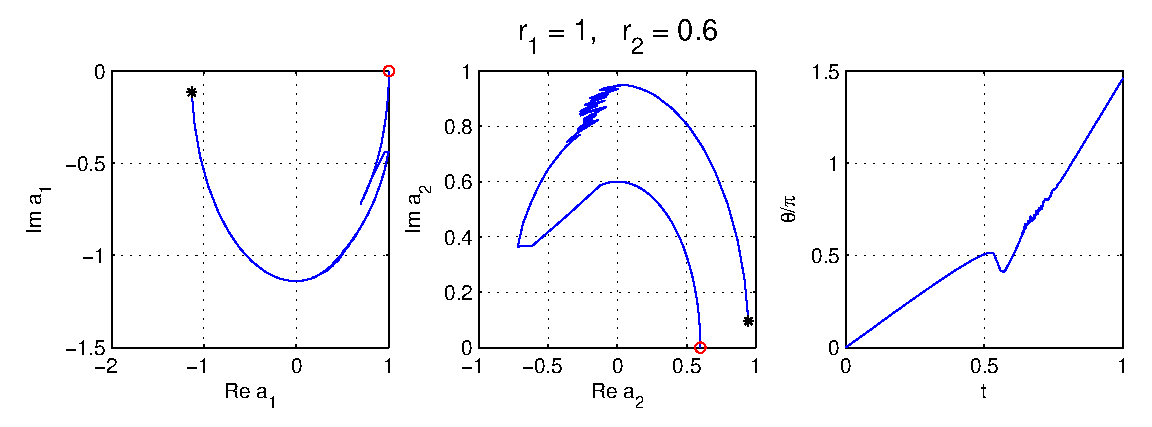
\includegraphics[width=\textwidth]{sliceflow5.eps}

until we get back the nice smooth solution:

\vspace{2ex}\noindent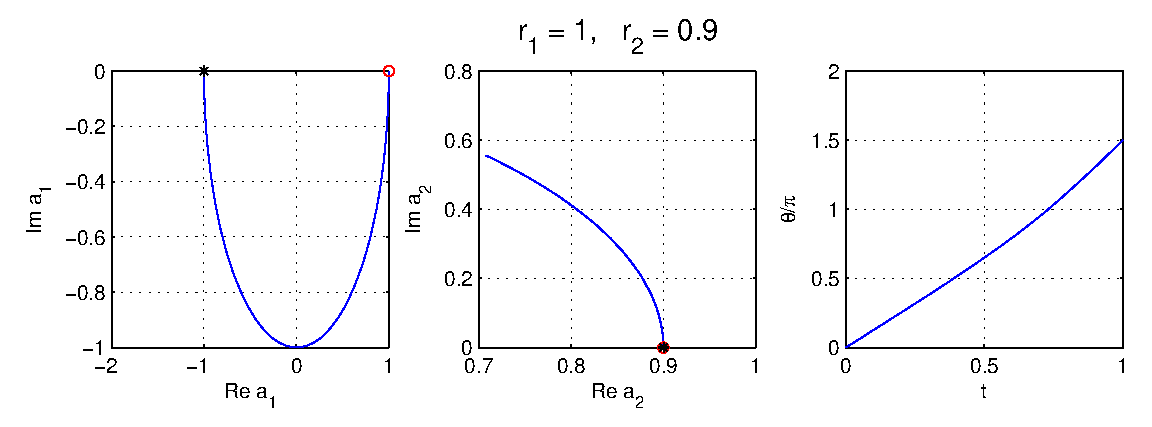
\includegraphics[width=\textwidth]{sliceflow6.eps}

which, however, is no longer periodic, while the shift is now $3\pi/2$.  This picture persists for all $r_2 > r_1$.

\vspace{2ex}\noindent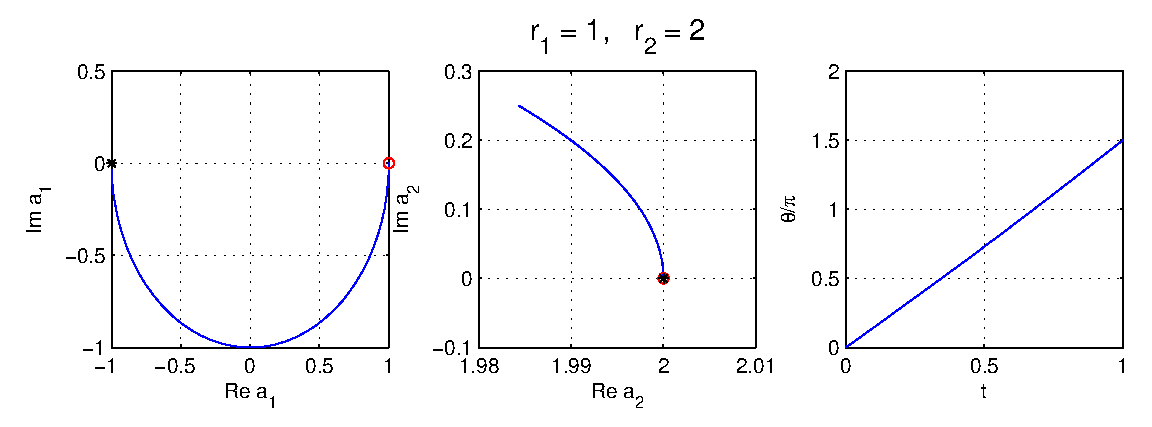
\includegraphics[width=\textwidth]{sliceflow7.eps}

So, it looks like the problem with the method of slices is not only due to running into the singularities,
but also due to the possibility of generating smooth orbits which go around those singularities
and generate wrong shifts without any indication that something has gone wrong.
These orbits are no longer periodic in the reduced space.  The only time this method works
reliably is when the flow is dominated by the first Fourier mode.  If this is not the case,
as in the KSE regime with multiple active modes, then we cannot expect that it will work.~~{\em Q.E.D.}

\vspace{2ex}
An old idea presented as a new one:  Why don't we define the dot product in the above equations as follows:
\beq
 a \cdot b = a_1 b_1^* + a_1^* b_1
 \,.
\ee{RLDfix}
Then, if I'm not mistaken, the whole thing reduces to my original idea for factoring out the $U(1)$
symmetry from the KS flow.  In this case we won't need to worry about running into, or moving around,
the singularities while generating spurious phases.  The only singularity will be at $r_1 = 0$,
which is trivial to deal with.

With the dot product defined as in \refeq{RLDfix},
\refeq{RLDrec} and \refeq{RLDred} become
\[
  \dot{\theta} = \omega_1
  \quad \mathrm{and} \quad
  \dot{\bar{a}}_k = i(\omega_k - k\omega_1) \bar{a}_k
\,.
\]
So they (obvious to Ruslan) do the job.


\subsection{2009-08-25 Eurosceptics do not like to slice}
\noindent{\bf Ruslan} (Predrag's translation) one gets a
phase shift by $\pi$ if one crosses the singularity.
\\
{\bf Ruslan} The shifts by $\pi$ is the least of my worries.
It is the fact that when $r_2 > r_1$ we get a nice smooth
solution of the reconstruction and reduced equations, yet we
get obviously wrong results.  I don't want to think why this
is happening.  I'd rather just stop using the approach where
such a thing can happen.
\\
{\bf Predrag} Your model illustrates why we need
monotonicity in phase (we are integrating 1d equation,
velocity cannot change sign?). But I think we will fix it -
it is like WKB for harmonic oscillator, one gets geometric
$\pi$ phase for each turn, and a neat way to do it is Maslov
trick - change slice at $\pi/4$, then change back at
$3\pi/4$, etc. Looks like something we can figure out. Sure
cute - getting semiclassical Keller-Maslow phase without
doing neither wave nor quantum mechanics. At least, not
consciously.

More interesting will be the phase for the method of
connections. If we are lucky, it is the same for relative
periodic orbits.
\\
{\bf Ruslan} We had the discussion about monotonicity some
time ago (see above).  I don't have anything more to add at
the moment.
\\
I don't know much about WKB, or Keller-Maslow
phase, but I would like to get away from generating all kinds
of fixes, like using random $\slicep$ or switching between
slices.

\medskip\noindent{\bf Predrag} 1st mode will not work. Actually,
what Ruslan has run into so far is the same problem you
(Evangelos) and Rebecca run into independently; he is
measuring angle in polar coordinates, where we also run into
$d\theta/dt$ divergence, and shifts by $\pi$.
\\
{\bf Ruslan} I disagree that 1st mode won't work, I think it
will. And I don't think using polar coordinates is the
problem.  Forget about dynamics.  Just look at functions
defined on a circle and ask yourself how to identify
functions that differ only by a shift.  My answer: The phase
of the 1st Fourier mode will give you the shift.  So just use
it to rotate the functions on top of each other.

\noindent {\bf Evangelos} Apart from quantum mechanics there
are classical systems that exhibit such behavior, see for
example
\HREF{http://prl.aps.org/accepted/L/cf079Ya5Q7f19828e08c7183313c1d9b2e9126ce4}
{this PRL paper}. I've only seen it in Hamiltonian systems,
where this behavior is called monodromy since one studies the
system as it goes once around a singularity (is the etymology
clear to non-Greeks too?). It apparently arises when a
function fails to be single-valued, which again should point
out why we need monotonicity in phase.\\
\textit{Question for Ruslan} Is it really trivial to deal
with the singularity at $r_1=0$?\\
{\bf Ruslan} Yes, but you should never ever try to
numerically integrate the reconstruction or the reduced flow
equations if you expect to get the correct reduced
representation of the orbits of the original flow.  Instead,
integrate the original flow and then pull the obtained orbit
onto the slice while keeping track of the shift you generate
while doing it.  If the original orbit goes exactly through
$r_1 = 0$ (within the round-off error), then add (or
subtract) $\pi$.  That's all.\\
{\bf Evangelos}  I agree that integrating the equation on the
slice is not the safest think to do. I would like to
understand where the spurious shifts that you have discovered
come from, though. It looks like the reduced space has a
branch cut and as one integrates the equations around the
singularity he finds oneself on a different leaf.

There is something I don't understand in the procedure you
describe here. Does the need to add or subtract $\pi$ come
from the fact that most implementations of $arg$ or $arctan$
functions do not distinguish quadrants? I do not understand
how else it is connected to crossing through $r_1 = 0$ or why
it does take care of the singularity. You can approach the
singularity through any direction on the $a_1$ plane, so the
way to overcome the singularity on a point with $r_1=0$ seems
to be to use the angle at which you approach to it (that you
get from the previous point) to correctly rotate it onto the
slice. The difficulty is that then you are not able to tell
where $\EQV{2}$ and $\EQV{3}$ lie on this space as they both
have $r_1=0$: their group orbits do not intersect your slice,
so you do need another ``coordinate chart'' to cover the
space.
\\
{\bf Evangelos} You still need to cover the reduced space
with more than one coordinate systems which is essentially
the same as choosing a new slice.\\
{\bf Ruslan} No. You don't need more than one coordinate
system.  Just use the Fourier modes as reduced coordinates,
with the phase of the 1st mode fixed.  The phase of the 1st
mode will be the reconstruction shift.\\
{\bf Evangelos} Even if this doesn't bother us, I am afraid
that we will get projections that are not more informative
than Figure 42 in todays' version of my thesis, where the
singularity was dealt with but $\EQV{2}$ and $\EQV{3}$
collapse to the same point.\\
{\bf Ruslan} I cannot guarantee that the pictures we get
will be nice and simple.  Of course, since the reduced space
is a semi-space (because $r_1 \geq 0$), the reduced orbits
may not always look pretty and smooth: They will have sharp
turns when they come close to, or hit, the $r_1 = 0$
subspace.  But at least when I look at orbits projected onto
Fourier modes, I know how to interpret them.  When I'm
looking at the projections onto some exotic curvilinear
coordinates, the pictures make no sense to me.\\
{\bf Evangelos} On the utility of Fourier modes as a
representation I disagree in two levels. I anyway find that
Fourier modes projection tell us very little about dynamics.
Wasn't this the reason to use different coordinate systems in
the KS paper? So as long we can construct dynamically
meaningful projections in the new variables I do not worry
how we got them.

Furthermore, what you describe above is equivalent to using
the invariants of Table 3 in Chapter 8 in my thesis. The new
coordinates are exactly the Fourier modes rotated back to the
slice defined by $\Im(c_1)=0$, this is how they were
obtained. The difference is that in Table 3 the singularity
is explicit. The important point though is that what you like
to see as a linear transformation is in fact a nonlinear
transformation through the dependance of the angle on the
point in space in which it is evaluated. Whereas in a linear
transformation all points in space are rotated by the same
angle. Therefore without knowing it you use exotic
curvilinear coordinates. The connection to the original
Fourier modes is that the magnitude in each Fourier plane
stays invariant. Of course things get even more exotic in my
thesis, but the motivation behind that was to get projections
that provide more information about the dynamics.

As a general comment, it appears that when we try to see the
reduced space as embedded in the original space, no matter
how we go from $N$ to $N-1$ dimensions we impose a
conservation law that did not exist in the original system
(as it was allowed to have motion in the direction of group
action) that restricts the motion to an $N-1$ dimensional
space which cannot in general be given a nice structure.

\subsection{2009-08-26 Eurosceptics carry the day}

\noindent{\bf Predrag} OK, now that Ruslan has gone on
strike I spent a day screwing around with Mathematica,
checked epicyclist formulas and reproduced Ruslan's graphs.
As I am using \texttt{NDsolve[\dots]} as a black box, I do
not get the same screwy details close to $(r_1,r_2)=(1,0.5)$,
but the result is the same - for $r_2$ sufficiently larger
than 1/2 one gets extra $\pi$ shift, with no integration hint
that one is going around a singularity. That is unacceptable.
As Ruslan expects,
random choices of complex (not real) \slice\ fixing
point $\sliceTan{}$ move the singularity around but are essentially no
help.

I will still try to use Maslov trick and switch the slice
whenever $\dot{\theta}$ starts misbehaving, but for that I
need to learn how to use \texttt{Method -> \{"EventLocator"}
within \texttt{NDsolve[\dots]}, but that sure looks like a
bitter pill. I do not mind having several slices as long as
the returns to (dynamical) Poincar\'e sections trace out
smooth unstable manifolds suitable to partitioning the
\reducedsp.

Marsdenites did not note this problem as they only applied
the method to \reqva, and there it is OK.

I agree that if one is to fix the \slice\ by one Fourier
mode, \refeq{RLDfix} is the most natural choice, and would be
easiest to explain in a publication. Unfortunately, we ran
into singularities when we tried it for \CLe\ in Siminos
thesis\rf{SiminosThesis} and
\HREF{http://ChaosBook.org/projects}
     {Rebecca's summer project}.
But Ruslan, please do give it a try.

\medskip\noindent{\bf Ruslan}
Actually, not really on strike, just reluctant to participate
in your, what I believe to be, futile efforts to apply all
kinds of fixes and patches to the approach which, I believe,
is fundamentally incurable when it comes to systems like KS
in a fully developed chaotic regime. [\dots]

\medskip\noindent{\bf Predrag} Fair enough - way too many fixes and
patches. We need to quotient the symmetry in order to figure
out the symbolic dynamics for KS and for plane Couette and
pipe flows. If something like \refeq{RLDfix} works it would
be nicer. The reason why we think it will not is that when we
use the polar coordinates-inspired \slice\ fixing point
$\ssp^{*}=(0+i,0, \cdots)$, $\Re\ssp_1=0,\;\\Im\ssp_1>0$
(which I believe for $U(1)$ version corresponds to fixing the
phase of the first Fourier mode) the \reducedsp\ equations
are given by
\beq
\dot{\ssp} = v - \frac{{\Im} v_1}{{\Re}\ssp_1} t(\ssp)
\,.
\ee{EqMotionMovFrame}
Trajectories shown in %\reffig{fig:PCunrot1}
Siminos thesis\rf{SiminosThesis} and
\HREF{http://ChaosBook.org/projects}
     {Rebecca's summer project}
exhibit jumps by $\pi$. With $\ssp^{*}$ on \reqv\ orbit we
were luckier, and got a strange attractor which encountered
no $\dot{\theta}$ singularity. But unhappy, as we did not
understand why we were lucky.

\medskip\noindent{\bf Predrag} to Evangelos when you tried my initial
proposal to project velocity locally (not on a global slice),
the method that when fixed will probably be called ``method
of connections'' - are you sure that the extra geometrical
phases gained by relative periodic orbits were not rational
fractions of $\pi$?

\subsection{2009-08-27 Don't worry. Be happy}

\begin{description}
\item[Ruslan]
    Let me start by answering Evangelos's question about rotation
by $\pi$.  Forget about multiple modes for the moment.  Just
consider evolution of the first mode: $a_1(t) =
r_1(t)\mathrm{e}^{i\phi_1(t)} \in \mathbb{C}$.  If $a_1(t)$
goes through zero, then $r_1(t)$ bounces off of zero, while
$\phi_1(t)$ changes by $\pi$ or $-\pi$, (the sign is
immaterial).   This is just the nature of the polar
coordinates and has nothing to do with the implementation of
$arg$.

\item[Evangelos]
But still I don't understand why would you need to add or subtract
$\pi$? Doesn't the function you use to calculate the angle in this
plane take care of that?

\item[Ruslan]
That's it.  All I was saying
was that $\phi_1$ would change by $\pi$ or $-\pi$ as $a_1$
crosses zero.  And that's what the angle function would give
you.  Nothing else needs to be added.

\item[Ruslan]
Now about the nature of what you call the 'singularity'.  If
I understand it correctly, what worries you is that, if we
take $\phi_1$ as our $\theta$, then each time it changes by
$\pi$, the $k$-th mode needs to be changed by $k\pi$, $k >
1$.  You perceive this as a jump, i.e. a discontinuity of the
reduced orbit, which you don't like.  Is this what you mean
by the 'singularity'? If `yes', then do you really need to
worry about it?

\item[Predrag]
If $1/x$ is considered a
`singularity' for $x=0$ on small islands off Continent, than
we will be so bold to call it singularity. As you say, there
should be simple analytic fixes for going through zero; we
have to make sure that we teach our numerical routines how to
implement this. Your pretty and clean epicycle model just
gave me a new set of ulcers, as for $r_2$ not very larger
than 1/2 the integrators seem not to know that there was any
singularity at all, and relative periodic orbits became
periodic only mod~$\pi$. And $\pi$ or $-\pi$  sign is not
immaterial - we have to get \rpo s shifts right.

\item[Evangelos]
I want to add that the singularities in expressions such as
in Table 3 in Chapter 8 of my
thesis cannot be essential, in the sense that, since the transformations
are generated by rotations, the expressions
cannot really blow up. In practice they pose numerical issues,
related to the small denominators in these expressions. So I agree there
should be simple analytic fixes.

\item[Ruslan]
If you think about it, what you perceive as a jump is
actually a very fast rotation (infinitely fast if you go
exactly through zero, but otherwise finitely fast).  If you
don't like that it rotates so fast, then why don't you just
rescale the time?  Just slow it down near $r_1 = 0$.  I think
something like $d\tau = dt/r_1(t)$ might work, since it will
remove $\Re\ssp_1$ from the denominator in
\refeq{EqMotionMovFrame}.

\item[Predrag]
Agreed. I have been also thinking about redefining time.
That's also in ChaosBook
\HREF{http://chaosbook.org/chapters/conjug.pdf} {Chapter 6 - Get straight},
called there the
Kustaanheimo-Stiefel (also known as KS!) transformation, and
applied in Example 6.2: what to do with Keplerian ellipses of
arbitrarily large velocity. That we might need for close
passages to the $U(1)$ invariant subspace, with $r^2 = \sum
\ssp_k^*\ssp_k$ going small. Fortunately, in KS that never
happens - strange attractor is safely away from the $u(x)=1$
\eqv. Our problem with method of slices is more naive, as you
explain above.

Of course, the real challenge is: who will be the first to read the
\\
\HREF{ChaosBook.org/projects/siminos/thesis.pdf}
      {Thesis that Nobody Reads} first?

\item[Ruslan]
On the other hand, if our goal is to eventually reduce the
dynamics to a Poincar\'e map, then why do we need to worry
about time at all?

\item[Predrag]
Agreed - anything that gets us the sensible return (or
forward) maps is good. Just have to make numerics is correct,
and yields correct \rpo s shifts and periods - at the moment
we do not know how to do that right even for the 2-mode
epicycles model.

\item[Evangelos]
I also agree, that was my thesis final conclusion on what one should do: just
make sure that the Poincar\'e section is away from problematic regions. It is
just that finding a good section is not always easy, so one needs some visualization
that works well in order to get intuition on where to place it.
\end{description}

\subsection{2009-08-28 On ulcers, singularities, and `tender beasts'}

\noindent{\bf Ruslan} I thought the dot product
\refeq{RLDfix} would cure your ulcers for the epicycle model,
and I'm pretty sure for the CL and KS as well, provided you
stop worrying about the fast rotations in the reduced space.
I don't mind that you call them `singularities', but, hearing
your complaints about numerics, I'm pretty sure somebody
does...  Let me tell you something about computers: they are
tender beasts and if you say, or even think, this word in
their presence, they will get spooked and throw all kinds of
fits.  But seriously, as I already said above, any symmetry
reduction or other transformations that you want to carry out
should be done as post-processing, i.e. after you obtain your
numerical trajectory by integrating the original flow.  That
way the singularities are much more tractable numerically.

\subsection{2009-08-27 Maslov trick}

\noindent{\bf Predrag}  The Maslov trick is described in
\HREF{http://chaosbook.org/version12/chapters/WKB.pdf}
{ChaosBook vers. 12, Chapter 31 - WKB quantization}.
Now I realize I give no references to Maslov paper or other
relevant sources - if you find them, please let me know so we can
write up the remark on the Maslov approach. Citing from this
chapter:

A simple physical picture, due to Maslov, is illustrated by quantization
of the harmonic oscillator. Semi-classical propagator has
a factor $1/$(velocity$)^{1/2}$, reminiscent of our $\dot{\theta}$, and
that blows up at the turning points, points where the particle as viewed
from the $q$ coordinate frame reverses velocity.

In the $q$ coordinate, the turning points are defined by the
zero kinetic energy condition,
and the motion appears singular.
This is not so in the full \statesp: the trajectory in a smooth confining
1-dimensional potential is always a smooth loop,
with the ``special'' role of the turning points $q_L, q_R$ seen to be an
artifact of a particular choice of the $(q,p)$ coordinate frame
(in our application, choice of a slice). Maslov's
idea was to proceed from the initial point
$(q',p')$ to a point $(q_{A},p_A)$ preceding the turning
point in the $\psi(q)$
representation, then switch
to the momentum representation (in our application, use a slice turned by
$90^o$)
continue from $(q_A, p_A)$ to $(q_B, p_B)$, switch back to the coordinate
representation (in our application, use a slice turned by
$90^o$), and so on.

In other word, as slices are local, switch to the next one whenever
convenient, and for recurrent orbits, make sure you are in the original
slice when you come back, in order to get a return map and hopefully sensible
symbolic dynamics.

\subsection{2009-08-28 Any 2-mode epicycle reduces to a periodic orbit}

\begin{description}
\item[Predrag]
A generic 2-Fourier modes epicycle trajectory runs on a 2-torus in the
full \statesp. Hence any trajectory is a \po\ in the \reducedsp, not
only the hand-crafted \rpo\ such as \refeq{RLDrec}.
(I actually verified this statement by running random trajectories
in \texttt{Mathematica}, so it is true.)
For testing methods of symmetry reduction
it might be a good idea to increase the number of Fourier modes.
\item[Ruslan]
That's right.  And thinking about it
as a 2-torus might hint at why the singularity develops as
$r_2$ grows. As $r_2$ grows, at some point the torus becomes
self-intersecting. I'm sure this happens when $r_2 = r_1/2$.
The SO(2) group orbit on this torus is a line that winds once
around $r_1$ and twice around $r_2$.  As the torus becomes
self-intersecting this orbit first self-intersects at $r_2 =
r_1/2$ and then forms a knot.  And that's why an extra $\pi$
shift appears when we try to project an orbit onto the slice
normal to this knot.  This is just a speculation, but maybe
there is something in it.
\end{description}

\section{2009-08-27 Symmetry reduction by method of connections?}

\noindent{\bf Predrag}
Here we take $t(\ssp)$ to
be the tangent for the trajectory state space point \ssp\ is
used \emph{locally}, within the `horizontal' hyperplane
normal to $t(\ssp)$.

The 2-epicycle model is a linear sum of Fourier modes
$(\ssp_{-2},\ssp_{-1},1,\ssp_1,\ssp_2)$.
Predrag's first guess for the reconstruction equation for
phase shift for slice fixed \emph{locally} by $t(\ssp) =
T\cdot\ssp(t)$ was
\beq
\frac{d\theta}{dt}=
     \frac{t(\ssp)^{*} \cdot \dot{\ssp}(t) + \dot{\ssp}(t)^* \cdot t(\ssp)}
                        {2 \,t(\ssp) \cdot t(\ssp)^{*}}
\,,
\ee{MethConnWrong}
which evaluates to
\[
\frac{\omega_1\, \ssp_1(t) \ssp_1(t)^{*}
  + 2\,\omega_2\, \ssp_2(t) \ssp_2(t)^{*}
     }{
               \ssp_1(t) \ssp_1(t)^{*}
  +         4\,  \ssp_2(t) \ssp_2(t)^{*}}
\,.
\]
This integrates to a convoluted, initial point dependent
but \po\ in the reduced
space, because in the 2-epicycle model all motion is on
2-torus in the full \statesp, 1-torus in the
$U(1)$-\reducedsp. The reconstruction equation
\refeq{MethConnWrong} appears to be wrong; I forgot to
include the `connection,' \ie, the effect of the frame itself
changing in the next time step. Presumably \stabmat\
needs to be included, as in the Lie algebra equivariance
condition
(see Siminos thesis\rf{SiminosThesis} and
\HREF{http://ChaosBook.org/projects}
     {Rebecca's summer project}).
For linear models \stabmat\ is constant, would be easy to
include into integrations.

If you want to be a path-breaking American type entrepreneur, rather
than a Eurosceptic kvetch, derive the right reconstruction equation
for this case. The glove is thrown.

\begin{description}
\item[Ruslan to Predrag]
I've never aspired to be an American entrepreneur.
I'm a lazy Ukrainian, so I don't do things unless I'm
convinced they are relatively easy to do and will result in
something useful.  Besides, I don't like algebra, not even of
Lie kind, not even of any kind.  I like geometry.  And the
vague picture I have in my mind tells me that the method of
connections, being in some sense more local than the method
of slices, has even less chance of succeeding where the
problems we are experiencing are clearly of a global nature.
So, I don't understand why I should be trying to work through
this quite complicated calculation, while I have a much
simpler approach based on the 1st Fourier mode, which works
for epicycles and I'm quite sure will work for KS.  It might
not give me a nice and smooth orbit.  The orbit might even
look ugly, but at least it will be a correct symmetry reduced
orbit.

\item[ to Ruslan]
OK, we'll suffer through
convoluted algebraic thinking as it applies to the geometry
of equivariant flows, and you industrious subject of Queen
Elizabeth go test \refeq{RLDfix}, the simple approach based
on the first Fourier mode, on KS.

\item[ to Predrag]
OK, this glove fits me better, especially since I've done most of it 20 months ago.
\end{description}

\section{2009-08-29 Kuramoto-Sivashinsky O(2) quotienting}

\subsection{Back to the future: pasting from 2007-12-31}

\medskip\noindent{\bf Ruslan pasting from siminos/blog/davidchack/071231fundamental.html}
To fix the notations, let me recap the Kuramoto-Sivashinsky
equation (KSE) and its representation in Fourier space:
\[ u_t = -uu_x - u_{xx} - u_{xxxx},  \quad x \in [-L/2, L/2] \]
with periodic boundary conditions:  $u(x+L,t) = u(x,t)$.  In the Fourier representation
\[ u(x,t)=\sum_{k=-\infty}^{+\infty} a_k (t) e^{ i q_k x }\,,\]
where $ q_k = 2\pi k/L$, the KSE takes the form
\[ \dot{a}_k = v_k(a) = (q_k^2 - q_k^4)a_k - \frac{iq}{2}\sum_{m=-\infty}^{\infty}
    a_m a_{k-m}\,,\quad a_k \in {\cal C}\]
It is convenient to represent complex modes as pairs of real
variables, either in cartesian or polar coordinates:
\[ a_k = (b_k, c_k) = b_k + ic_k = (r_k, \theta_k) = r_k e^{i\theta_k}\,. \]

\noindent{\bf Symmetries:} If $u(x,t)$ is a solution of the KSE, then so are
\[ \tau_{\shift/L} u(x,t) = u(x+\shift,t) \quad\mbox{and}\quad R\,u(x,t) = -u(-x,t).\]
The action of symmetry transformations on Fourier modes is as follows:
\[ \tau_{\shift/L} a_k = e^{iq_k \shift} a_k = (r_k, \theta_k + q_k \shift) \,,\qquad R\,a_k = -a_k^\ast = (-b_k, c_k)\,.\]

\subsubsection{Defining KSE quotient space $\pS/$O(2)} % (a.k.a. fundamental domain)}
\label{sect:RLDslice}

The KSE quotient space $\pS/$O(2) is defined in Fourier space as follows:
\begin{enumerate}
\item If $r_1 > 0$ then $\theta_1 = \pi/2$ and $\dot{\theta}_1 \leq 0$;
\item if $r_1 = 0$ then $\arg \dot{a}_1 = \pi/2$;
\item if $a_1 = \dot{a}_1 = 0$ then the KSE solution lives in
        the $L/2$-periodic invariant subspace, where $\pS/$O(2) is
        defined as above but for the 2nd mode;
\item and so on...
\end{enumerate}
So the quotient space $\pS/$O(2) consists of a hierarchy of
slices fixed by the $k$-th Fourier mode for the
$L/k$-periodic invariant subspace.

\begin{description}
\item[Predrag's comment] I do not find fixing a single
Fourier coefficient natural, and you pay for it by having to
deal with discrete shift symmetry subcases separately (fixing
higher $k$ Fourier coefficients).
\item[Ruslan's reply] I think it is completely natural that
for solutions symmetric by $L/k$ shift, we use the $k$-th
Fourier mode. Since functions in $L/k$-symmetric subspace are
invariant under KS dynamics, using $k$-th Fourier Mode in
$[0, L]$ is the same as using the 1st Fourier mode in $[0,
L/k]$.  Also note that, again because of the invariance of
these subspaces, the choice of the mode which defines
$\pS/$O(2) is fixed once and for all times by the initial
condition, so there is no need to jump between slices when
following the KS flow.
\end{description}

\subsubsection{Mapping KSE solutions to $\pS/$SO(2)}

Following Predrag's suggestion, I'll split the mapping of KSE solution to $\pS/$O(2) into two parts:
1) map to $\pS/$SO(2) by translation $\tau_{\shift/L}$; 2) map from $\pS/$SO(2) to $\pS/$O(2) by reflection $R$.

\medskip\noindent{\em ...to be continued...}

%\vspace{2ex}\noindent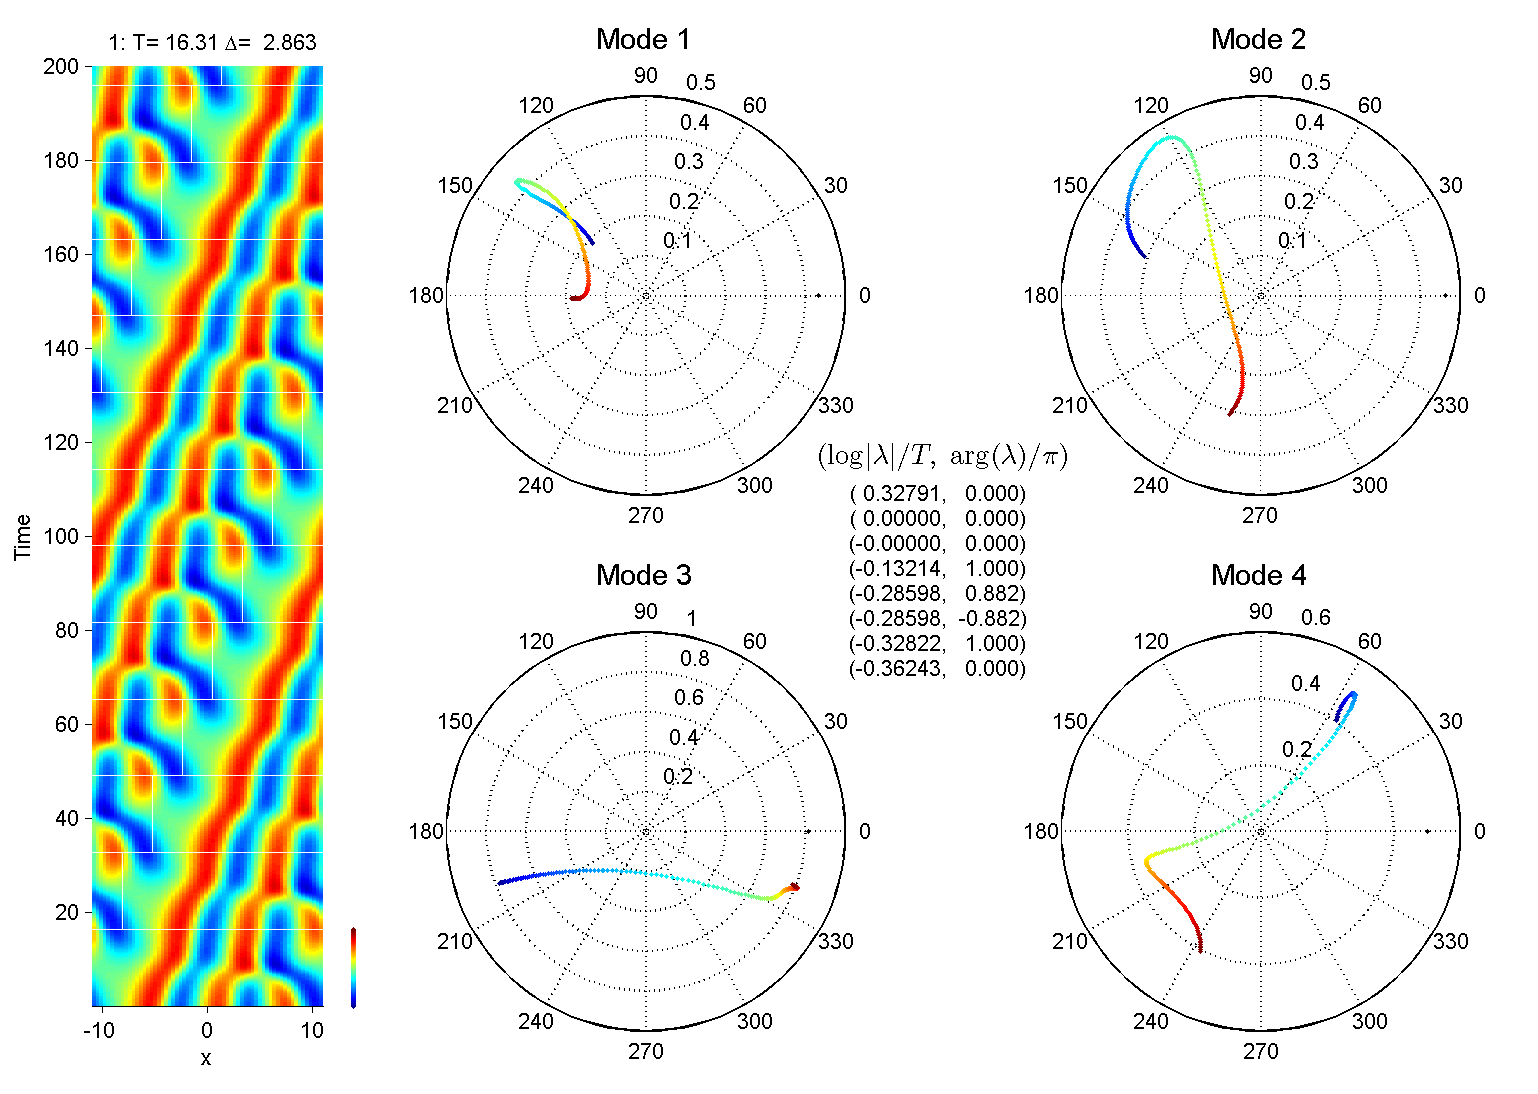
\includegraphics[width=\textwidth]{ks22rpo016.31_02.863.pdf}


%
% *Note 1:* The invariant subspace of antisymmetric solutions
%
% $$ u(x,t) = R\,u(x,t) = -u(-x,t) \quad\Rightarrow\quad Re\,a_k = 0 $$
%
% belongs to the FD.
%
% *Note 2:* If both
%
% $$ a_1 = 0 \mbox{~~and~~} \dot{a}_1 = 0 $$
%
% then the solution lives in the L/2-periodic invariant subspace, and the FD
% is defined in terms of
%
% $$ r_2 \mbox{~~and~~} \theta_2\,. \mbox{~~And so on...} $$
%
% A KSE solution
%
% $$ (r_1, \theta_1, r_2, \theta_2, \ldots) $$
%
% is mapped into the FD by translation
%
% $$ \shift/L = \frac{\pi/2 - \theta_1}{2\pi} $$
%
% and reflection if
%
% $$ \dot{\theta}_1 > 0\,, \mbox{~~or~~} b_1\dot{c}_1 - c_1\dot{b}_1 > 0\,, \mbox{~~since} $$
%
% $$ \dot{\theta_k} = \frac{b_k\dot{c}_k - c_k\dot{b}_k}{b_k^2 + c_k^2} $$
%
% The map into FD is characterized by two parameters: the translation
% parameter
%
% $$ \shift = \frac{\pi/2 - \theta_1}{2\pi}L $$
%
% and the reflection parameter
%
% $$ \rho = 1 \mbox{~~when~~} \dot{\theta}_1 \leq 0 \mbox{~~and~~} -1
% \mbox{~~when~~} \dot{\theta}_1 > 0 $$
%

\subsection{2009-08-31 A closer look at the singularity}

\noindent{\bf Evangelos}
Taking \CLe\ as an example I will examine how the invariants
\beq
\begin{split}
        \overline{x}_2 &= \sqrt{x_1^2+x_2^2} \continue
        \overline{y}_1 &= \frac{x_2 y_1-x_1 y_2}{\sqrt{x_1^2+x_2^2}}\continue
        \overline{y}_2 &=\frac{x_1 y_1+x_2 y_2}{\sqrt{x_1^2+x_2^2}}\,.
        \label{eq:invLaser}
\end{split}
\eeq
generated by straightforward application of the moving frame method behave as $x=x_1+i x_2$ approaches
zero. For the limit to exist we must get a direction independent result as $x\rightarrow 0$.
Using $x=r_x\, e^{i\theta_x}\,,\, y=r_y\, e^{i\theta_y}$ we can write, for instance, $x_2 y_1-x_1 y_2 = r_x r_y \sin(\theta_x-\theta_y)$
and therefore,
\beq
        \overline{y}_1= r_y\sin(\theta_x-\theta_y)\,.
\eeq
Therefore, for any given $y$, the limit of $\overline{y}_1$ for $x \rightarrow 0$ does not exist, as the above expression depends on the direction
on the complex $x$-plane along which we approach zero. In terms of projecting dynamics on variables \refeq{eq:invLaser} (or applying the equivalent
procedure of rotating points back to the \slice) this means that
we need to take into account the direction along which
we approach zero and use the `angle
of descent' as the angle with which we rotate points back to the \slice, if such points have exactly $x=0$ (in CLE this does not happen). Since the subspace $x=0$ is not flow invariant we do not need to worry about dynamics that stay within the subspace. We need to worry about the equilibria that exist in this subspace though, here the equilibrium at the origin, as there is no way to transform them to the new variables. For KS $\EQV{2}$ and $\EQV{3}$ belong to such a subspace.

\begin{description}
\item[Ruslan's more optimistic view of the singularity] Of
course, when $x = 0$, the angle $\theta_x$ is undefined.  But
if you look dynamically at $x(t)$ as it crosses zero at $t =
t_0$, then you realize that if $\theta_x(t < t_0) = \theta$
then $\theta_x(t > t_0) = \theta + \pi$ and all you need to
decide is how to define $\theta_x(t_0)$.  The most natural
definition is based on the direction of $\dot{x}(t = t_0)$,
i.e. $\theta_x(t_0) = \arg \dot{x}(t_0) = \theta + \pi$.
That's the reason I have item 2 in my definition of $M/$O(2)
quotient space.  So, as you can see, $\theta_x(t)$ remains
well defined at all times.

Regarding E2 and E3 in KS, they live in $L/2$- and
$L/3$-periodic subspaces, respectively.  So, to map them onto
$M/$O(2), we'll use the 2nd and 3rd Fourier modes,
respectively, as stated in items 3 and 4.

\item[Evangelos]
I agree about trajectories that cross zero, but not about
\EQV{2} and \EQV{3}. As soon as you use 2nd and 3rd Fourier
modes you effectively use different transformations, so it is
not obvious to me how you can piece everything together in
the same space. Fortunately we are not interested on dynamics
in $L/2$- and $L/3$-periodic subspaces, as they are not
invariant, but rather on how unstable manifolds of \EQV{2}
and \EQV{3} organize the $L$-periodic space. As those
unstable manifolds do not have vanishing first Fourier mode
we can visualize them and forget the equilibria.

\item[Ruslan]
  Actually, it's somewhat the other way
around for me: what worries you, does not worry me and vice
versa.  The proposed hierarchy of transformations is
completely consistent, since the higher-mode transformations
only act on those {\statesp} points which are not influenced
by the 1st mode transform.  By the way, the $L/k$-periodic
subspaces \underline{are} invariant: e.g. if $a_1(0) = 0$ and
$\dot{a}_1(0) = 0$ then $a_1(t>0) = 0$, so the solution is
$L/2$-periodic (provided $a_2(0) \neq 0$).  And finally, we
do have to keep track of the special symmetries of the
unstable manifolds of the equilibria.  For example, once
$\EQV{2}$ is placed within $M/$O(2) using the 2-nd Fourier
mode, its unstable manifold completely lives in the
anti-symmetric subspace (i.e. $Re\,a_k = 0$). {\color{blue}
The 1st mode transformation doesn't do anything to it, since
for any point on the manifold $\theta_1 = \pi/2$ already.}
So, the manifold we show in our SIADS Fig.~5.6 is already in
$M/$O(2).  What worries me is that $\EQV{2}$ is represented
here by two different points ($\EQV{2}$ and
$\tau_{1/4}\EQV{2}$).  This is the result of the additional
symmetry of $\EQV{2}$.  Whether or not these two points can
be merged into one $\EQV{2}$ without loss of dynamical
information about the KS flow, remains to be investigated.

What I wrote above, highlighted in blue, is wrong.  SO(2)
still acts in the antisymmetric subspace, since the points
there can also have $\theta_1 = -\pi/2$.  So they are rotated
by $\pi$.  Whether or not this will also rotate
$\tau_{1/4}\EQV{2}$ into $\EQV{2}$ I'm not yet sure.

\item[Evangelos]
SO(2) does not act in the antisymmetric subspace (in the
sense that it does not leave it invariant as a set) but
merely on the intersection of antisymmetric subspace and its
$\tau_{1/4}$ translated copy. The group orbits of points on
antisymmetric subspace produce a family of copies of it. One
can identify a single representative by choosing for instance
$\theta_1=\pi/2$, so I don't see any problem with points on
the unstable manifolds of $\EQV{2}$. $L/k$-periodic subspaces
\underline{are not} invariant: if $a_1(0)=0$ then in general
$\dot{a}_1(0)\neq 0$, due to the nonlinear terms. Right?

\item[Ruslan]
  I didn't quite understand your
comments about the translated copies of the antisymmetric
subspace, but if you think it's not causing any problems, I'm
happy.  Regarding the $L/k$-periodic subspaces, I guess I
wasn't defining them correctly.  So, if $\dot{a}_1 \neq 0$
then we can still map this point to $M/$O(2) using the 1st
mode.  I was speaking then about the parts of $L/k$-periodic
subspaces which remain invariant under the KS flow.  They
need to be mapped to $M/$O(2) using higher FMs.

\end{description}


\subsection{2009-08-29 - Implementation of Ruslan's $a_1$-fixed slice}

\noindent{\bf Evangelos}
I thought its time to shut up and compute something, so I've
implemented first part of (my interpretation of) Ruslan's
prescription for KS that should take care of $SO(2)$. Namely,
I have fixed the \slice\ following
the rules of \refsect{sect:RLDslice}:
\bea
\Im \bar{a}_1  &=& 0
\continue
\mbox{If } r_1 &>& 0\,,\quad \mbox{\ESedit{rotate to the \slice\ by}}
        -\arctan( \Im a_1/\Re a_1 )
\continue
\mbox{If } r_1 &=& 0\,,\quad \mbox{\ESedit{rotate to the \slice\ by}}
        -\arctan( \Im \dot{a}_1/\Re \dot{a}_1 )
\,.
\label{ES-RLDslice}
\eea


\begin{figure}
 (a)~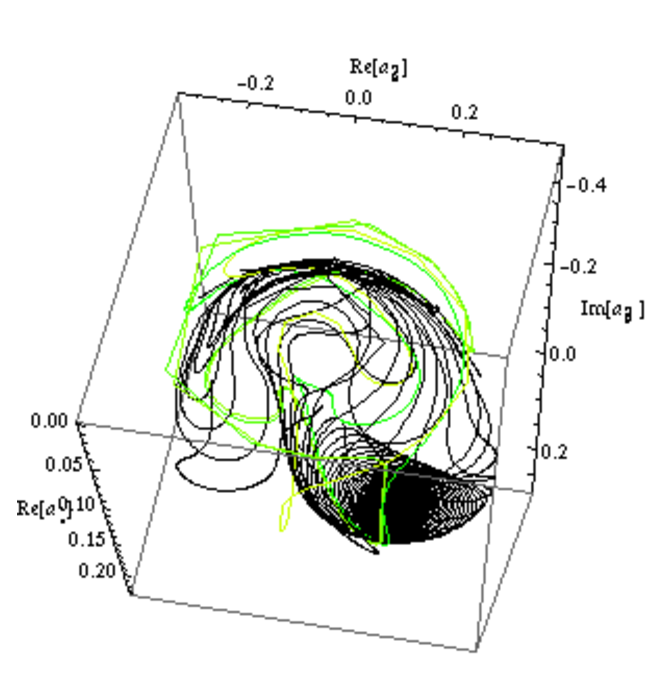
\includegraphics[width=0.45\textwidth]{ksRotatedTW1um.eps}\,
 (b)~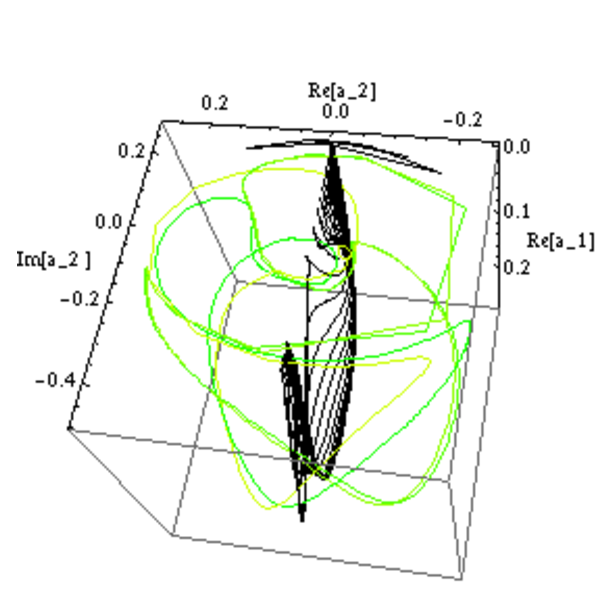
\includegraphics[width=0.45\textwidth]{ksRotatedE2um.eps}
\caption{
 $(\Re \bar{a}_1,\,\Re \bar{a}_2,\Im \bar{a}_2)$ projections of KS
 $\SOn{2}$-reduced dynamics by slice \refeq{ES-RLDslice}.
 Several \rpo s are shown along with the
 unstable manifolds of (a) \REQV{+1}, (b) \EQV{2}. $L=22$.
}
\end{figure}

I've posted such a figure long ago in Jonathan's blog, but
nobody got interested. I am also not happy with this figure
but one might argue that there are implementation problems,
and this is probably right, so I will have a second look.
Then, if I am to follow Ruslan's next step in the
prescription and set $\Im \bar{a}_2 =0$ in order to include
$\EQV{2}$ in this figure, the equilibrium will not ``meet''
it's unstable manifold, correct?

\begin{description}
\item[Ruslan]
 I agree that the unstable manifold of $\EQV{2}$ reduced by
 the 1st mode to $\pS/\SOn{2}$ will not meet $\EQV{2}$ reduced by
 the 2nd mode. \par I have a question: do we expect that an
 antisymmetric solution of KS will remain antisymmetric in
 $\pS/\SOn{2}$?  If yes, then we are in trouble, which has
 nothing to do with using the 1st mode: As I stated above,
 the only thing SO(2) can do to leave an antisymmetric
 solution antisymmetric is rotate it by $\pi$.  However, in
 order for the unstable manifold of $\EQV{2}$ (which is
 antisymmetric) to return to back to $\EQV{2}$ we need the
 rotations along the orbit to add up to $-\pi/2$ (to
 compensate for the $\tau_{1/4}$ shift).  So, somewhere along
 the way the unstable manifold has to leave the antisymmetric
 subspace.  This doesn't seem natural, since antisymmetric
 subspace is invariant under KS flow.

\item[Evangelos]
If we all agree that rotating points back to the slice $\Im\
a_1=0$ is equivalent to transformations of Table 3 in Chapter
8 in my thesis (that I copy here for convenience), up to
treatment of points with $a_1=0$, then my answer would be as
follows: applying reflections generated by $b_i\mapsto - b_i$
to the $u_i$ of \reftab{tab:SO2n6} we have $u_3\mapsto -u_3$,
$u_4\mapsto u_4$, $u_5\mapsto u_5$, $u_6\mapsto -u_6$ and so
on, so that the reflection matrix $\mathbf{R}$ in new
coordinates is diagonal, with entries $\pm 1$ and therefore
satisfies $\mathbf{R}^2=1$, as it should. Points in the
antisymmetric subspace $b_i=0$ for every $i$, are mapped to
points in the new coordinates that only depend on the $c_i$'s
and are therefore invariant under reflections, \ie,
antisymmetric. I don't see why the unstable manifold in
reduced space should leave the antisymmetric subspace, since
we don't even know were the equilibria live in such a reduced
space.

\item[Ruslan]
Well, we do know that the unstable manifold of $\EQV{2}$
converges to $\tau_{1/4}\EQV{2}$.  And I also assume that we
want $\EQV{2}$ and $\tau_{1/4}\EQV{2}$ to be represented by
the same point in the reduced space.  So, in order to bring
these two points together in the reduced space, we need to
rotate $\tau_{1/4}\EQV{2}$ by $-\pi/2$.  This rotation needs
to occur somewhere along an orbit (a closed loop in the
reduced space) within the unstable manifold of $\EQV{2}$.
But since the antisymmetric subspace is \underline{not}
invariant wrt rotation by $-\pi/2$, the orbit must leave the
antisymmetric subspace.  Another way to put this, is that, if
we only look at KS solutions within the antisymmetric
subspace, then $\EQV{2}$ and $\tau_{1/4}\EQV{2}$ are two
\underline{distinct} equilibria, since the first one is
unstable, while the second one is stable.  So, there is no
way to map these two equilibria into the same point while
staying within the antisymmetric subspace.

I don't know how much we should care about this, but this
tells me that, no matter how we construct the reduced space,
we will not be able to retain the simple structure of the KS
invariant subspaces within the reduced space.

\item[Ruslan 2009-10-14]
I still don't see how to reconcile this: On the one hand, it
would appear natural that the antisymmetric subspace should
be a part of $\pS/\SOn{2}$, but, on the other hand, the
antisymmetric subspace contains two distinct images of
$\EQV{2}$, while, in the reduced representation of the full
KS flow, we would hope that there would be only one point for
$\EQV{2}$ in $\pS/\SOn{2}$.  I can see only two possibilities
here: either we introduce discontinuities of the flow in
$\pS/\SOn{2}$ (like it is happening with my Fourier modes
representation), or we collapse the dynamics to a subspace
that completely ignores the phase information (e.g., like in
the energy transfer representation).

\item[Predrag 2009-10-15]
Yes, please quotient the full $\pS/\On{2}$. It's good to do so,
quotienting discrete symmetries helps a lot, see
\\
\wwwcb{/chapter/discrete.pdf}.

\item[Ruslan 2009-10-14]
Since I don't like collapsing things (I would like to have a
representation where I can keep track of the phase shift
$\theta$, which will allow me to reconstruct the original
dynamics if I wish to do so), and since I don't know how to
get rid of the discontinuities otherwise, I'm going to go
crazy and embrace them.  So, my plan here is as follows:
I'll try to construct a reduced representation (and hopefully
a Poincar\'e map) for the dynamics in the vicinity of the
unstable manifold of $\EQV{2}$. I think that if I manage to
do it here, then there is hope that it can be done for the KS
flow elsewhere as well.  I may continue using the Fourier
modes, or I might try something else, like using the
real-space representation (remember those $u$-$u_x$-$u_{xx}$
plots?).

\item[Predrag 2009-10-15]
You keep track of discrete $\LieEl$ for a given full
\statesp\ trajectory by noting every time you need to apply
it, upon exit from the fundamental domain, see Lorentz flow
$\pS/\Ztwo$ Van Gogh attractor in
\wwwcb{/chapter/discrete.pdf}.


\item[Evangelos to Ruslan]
Sorry that it took so long to get back to you, I am
just not sure I follow your arguments and I am afraid there
is a danger that the discussion becomes cyclic. The
antisymmetric subspace is indeed not invariant under $\pi/2$
rotations. On the other hand the image of the unstable
manifold of \EQV{2} under symmetry reduction by
\refeq{ES-RLDslice} is unique. It belongs to a
``antisymmetric set" in the reduced space, in which space the
action of reflections has been properly re-defined as in my
previous post. Of course the latter set is not invariant
under the action of reflection as defined in the original
space. In other words, if we would like to see the reduced
space as embedded in the original space we would have to say
that the linear antisymmetric subspace has been deformed in a
nonlinear manner through the transformations in
\reftab{tab:SO2n6} and reflections no longer leave it
invariant. Then I do not see any problems with identifying
all copies of \EQV{2} with a single point. I just see greater
problems with a discontinuous $\pS/\SOn{2}$.

Regarding ignoring phase information. I think we both agree
that it is safer to integrate only in the original space. So
no matter how we construct the reduced space we do not need
to through away any information.


\item[Ruslan to Evangelos 2009-10-14]
I think you nailed it: The transformations that identify all
copies of \EQV{2} with a single point do not appear to
respect the reflection symmetry.  If that's the case then how
can you call it an 'antisymmetric subspace', if it's not
invariant under reflections?  I thought that this is how we
define the antisymmetric subspace in the first place (i.e.
that it's invariant under reflections).  Is it not so?


\item[Evangelos: 2009-10-16]
I call it antisymmetric only because points in the original antisymmetric subspace are mapped to it. The correct term would be the fixed point subspace of reflections $\hat{\Refl}$ in the reduced space with coordinates $u_i$, where now reflections $\hat{\Refl}$ are not defined in the same way they are for the Fourier modes, but rather as in my post of 2009-08-29. Perhaps it might help to have a look at \reffig{fig:SO2inv}(a). There we can see that we still have reflection symmetry. For instance the traveling waves come in pairs. Points on the antisymmetric subspace are mapped on points with $u_3=0$ in this projection.
Of course this is a projection on a modified set of invariants, but the idea is the same.


\item[Ruslan: 2009-10-17]
OK, now I see where we differ.  I was hoping, maybe naively, to find, for any $u(x) \in \pS$, a unique shift $\theta(u)$ such that $\tau_{\theta(u)} u(x) = u(x - \tilde{L}\theta(u)) \in \pS/\SOn{2}$.  I was also hoping that the shift could be chosen such that $\theta(u) = 0$ (or $\pi$) for an antisymmetric $u(x)$.  That's what I meant when I was saying that my hope was that the antisymmetric subspace would belong to $\pS/\SOn{2}$.

The phase of the 1st Fourier mode is doing the job quite well, until we get to the point where $r_1 = \dot{r}_1 = 0$.  There I though I could use the 2nd Fourier mode, but encountered the problem when looking at the unstable manifold of \EQV{2}.  This manifold is antisymmetric, but it links two points of \EQV{2} shifted by $\pi/2$ with respect to one another.  So, I cannot construct $\theta(u)$ such that $\theta(u) = 0$ (or $\pi$) in the antisymmetric subspace and which identifies all \EQV{2} with a single point in $\pS/\SOn{2}$.  And that's my dilemma...

\end{description}


\begin{table}[t]
\caption
{First $11$ fundamental invariants for the standard action
  of SO(2)}
\scriptsize
\[
\begin{array}{ll}
  u_1=r_1=\sqrt{b_1^2+c_1^2}&  \\ u_3=\frac{b_2 \left(b_1^2-c_1^2\right)+2 b_1 c_1 c_2}{r_1^2}&u_4=\frac{-2
b_1 b_2 c_1+\left(b_1^2-c_1^2\right) c_2}{r_1^2}\\ u_5=\frac{b_1 b_3 \left(b_1^2-3 c_1^2\right)-c_1 \left(-3
b_1^2+c_1^2\right) c_3}{r_1^3}&u_6=\frac{-3 b_1^2 b_3 c_1+b_3 c_1^3+b_1^3 c_3-3 b_1 c_1^2 c_3}{r_1^3}\\ u_7=\frac{b_4
\left(b_1^4-6 b_1^2 c_1^2+c_1^4\right)+4 b_1 c_1 \left(b_1^2-c_1^2\right) c_4}{r_1^4}&u_8=\frac{4 b_1
b_4 c_1 \left(-b_1^2+c_1^2\right)+\left(b_1^4-6 b_1^2 c_1^2+c_1^4\right) c_4}{r_1^4}\\ u_9=\frac{b_1
b_5 \left(b_1^4-10 b_1^2 c_1^2+5 c_1^4\right)+c_1 \left(5 b_1^4-10 b_1^2 c_1^2+c_1^4\right) c_5}{r_1^5}&u_{10}=\frac{-b_5
c_1 \left(5 b_1^4-10 b_1^2 c_1^2+c_1^4\right)+b_1 \left(b_1^4-10 b_1^2 c_1^2+5 c_1^4\right) c_5}{r_1^5}\\ u_{11}=\frac{b_6
\left(b_1^6-15 b_1^4 c_1^2+15 b_1^2 c_1^4-c_1^6\right)+2 b_1 c_1 \left(3 b_1^4-10 b_1^2 c_1^2+3 c_1^4\right) c_6}{r_1^6}&u_{12}=\frac{-2
b_1 b_6 c_1 \left(3 b_1^4-10 b_1^2 c_1^2+3 c_1^4\right)+\left(b_1^6-15 b_1^4 c_1^2+15 b_1^2 c_1^4-c_1^6\right) c_6}{r_1^6}\\
\end{array}
\]
\label{tab:SO2n6}
\end{table}

\section{2009-10-20 Blogging on}

\begin{description}
\item[2009-10-20 Predrag] Moved Lyapunov stuff to
    \refchap{s:LyapunovVec}

\item[2009-10-28 Evangelos to renormalization experts]

One of my border ideas: Repeat the process that led to the
invariants of \reftab{tab:SO2n6} in each irreducible subspace
$i$, \ie, apply the moving frame method by setting $c_i=0$ for
each $i$, producing invariants $u_k^i$ where $k$ labels
coordinates. Then $\sum_k u_k$ will be a set of linearly
independent invariants. We would be able to map all equilibria
to unique points in this basis if it where not for the
singularities at $b_i=c_i=0$ for every $i$. So we will need to
follow a regularization procedure to remove it, but it might
now be done in a more natural way than simply manipulating the
denominator. It just reminds me of procedures in which each
term in a sum diverges but the sum can be regularized. Fels and
Olver\rf{FelsOlver99} use regularization techniques for group
actions but it is too technical for me.

The practical problem is that I do not get the simplifications
that led to simple expressions in \reftab{tab:SO2n6} when I try
to apply the moving frames method with $i>1$, I have no idea
why. So in thesis I add in appropriate places the invariants we
know that we will always get, \ie\ the Fourier magnitude in
each subspace.

\item[2008-11-20 Predrag] Idea: a conserved quantity $\to$
continuous symmetry. Can one use Noether theorem?
[2010-01-07 Predrag incorporated in ChaosBook]

\item[2008-11-20, 2009-10-29  Evangelos] I think that we
unfortunately cannot use it for dissipative systems. Noether's
theorem applies provided we can formulate the system as a
variational problem. It has caused me a great deal of confusion
tending to think of symmetries in this Noetherian way even for
dissipative systems. Some recent progress(?) beyond Noether's
theorem is summarized by Bluman\rf{Bluman07} in
\arXiv{math-ph/0511035}. See also \refref{BlumanAnco02}.

\item[2009-10-31 Predrag] Bluman\rf{Bluman07} seems to be a clear
and useful reference. Noether
theorem requires that equations of motion be cast in Lagrangian form,
and that the Lagrangian exhibits variational symmetries.
Variational symmetries are hard to find. For a system of equations
to be variational in form requires that their number is even,
that its linearized system (Fr\'chet derivative) is self-adjoint,
and that the system is non-dissipative. Bluman gives examples of some
of the usual tricks to recast the system in variational form, and
then circumvents it altogether. Then he discusses how to work without
Lagrangians, but whether this could be of use to us is not at all obvious;
most unlikely. It would have already been done for KS, if there
was something to do...

\item[2009-10-30 Predrag] An idea(?). In all ``Lyapunov
analysis'' workshop contributions of \refsect{iscpif} the
isolated hyperbolic eigenvalues appear in multiplets which
reflect the symmetry of the dynamics; doublets for KS, quartets
for complex Landau-Ginzburg, singlets to quartets for the
2-dimensional hard ball gasses, depending on the number of
translational symmetries. Due to the nonlinearities, they are
not exact multiplets, and in the ``physical'' spectrum they are
mixed up. What happens if we compute the Floquet eigenvectors
in the \reducedsp\ $\pS/\Group$? That has no symmetry, and thus
no multiplets? Perhaps the \monodromyM\ factors the way it
factors for the \Fd s of evolution operators (as in the famed
unpublished paper, still not understood by anyone but its
author)?

\item[2009-10-30 Predrag] Kalman filters were extensively
    discussed in ``Lyapunov analysis'' workshop weathermen
contributions of \refsect{iscpif}, and in many
other places - perhaps . They are a clever way
(at the level of assuming that noise is Gaussian) of
including partial observations into predictive models. Here
is why we might need them: in pipe flows, the 3-dimensional
velocity field is measured instantaneously by PIV in a
2-dimensional section across the pipe, not in a
3-dimensional volume. We might be able to make flow
stream-wise stationary by quotienting down-stream
translational invariance. That still leaves us with a
2-dimensional observation; while a simulation computes
90,000 discretization of the flow, this is -let's say-
3,000 points section of it, seems insufficient to identify
the state of the flow and start computationally predicting
what happens next. However, as the flow is confined to a
much lower-dimensional manifold, measuring the evolution of
the section in time should enable us to identify the state
of 3-dimensional flow. From then on the turbulent flow is
predictable for some finite time horizon controlled by the
Lyapunov exponents and vectors, with instantaneous state of
the fluid corrected by a 2-dimensional section observation,
folded into the flow by a Kalman filter.

\item[2009-10-31 Evangelos] Added
\begin{quote}
    siminos/rpo\_ks/davidchack/orbits/00README.txt
\end{quote}
    with Ruslan's instructions on how to read his data
    files with \rpo s and pre-\po s.

\item[2009-10-31 Evangelos to Ruslan] I see $10^4$ \rpo s
    of each kind. Are there any extra short orbits in the
    rest $4 \times 10^4$ that you have?

\item[2009-11-09 Predrag]
Modified
  book/chapter/continuous.tex ,
  book/chapter/discrete.tex, ...
- incorporated many wise Wirzba suggestions.

Not a cheerful development - to keep Evangelos happy, I now call the
 group of a symmetries of a given periodic orbit a `stabilizer'. Yech.
 Also, it feels like I have now spent 2 years writing up two group theory
 chapters and they are still in flux...

\item[2009-11-09 John FG]
    I've always hated the term `group orbit,' likely for similar reasons.

\item[2009-11-09 Predrag]
Group orbit I have gotten used to, cannot think of anything descriptive that would be better;
time and continuous symmetries are on collegial, Lie group setting, so thinking of an orbit as
$(N+1)$-dimensional is OK with me.

Other setback. I derived a co-moving slice, method of
connections reduced state-space `reconstruction' equation for
Andreas. The advantage would be that it never encounters these
annoying singularities of fixed slices. It is cute, it depends
on $\dot{v}$ (acceleration).

Unfortunately, every time I continue the calculation, three
attempts so far, $\dot{v}$ cancels out (it should do that in
Evangelos thesis calculation for \reqv\ slice too)? and I end
up with the simple `reconstruction, equation that I derived
earlier, for which Evangelos showed that it accrues
'geometrical phase.' And who the hell needs that.

For the life of me I cannot understand Marsden 'adjoint action'
formulation of the 'method of connections.' Andreas might, he
seems comfortable with the lingo.

\item[2009-12-03 Predrag] Went to Bonn, Andreas would not hear
another word from me about the 'method of connections.' Home
alone, again...

\renewcommand{\LieEl}{\ensuremath{g}}  % Predrag Lie group element
\renewcommand{\gSpace}{\ensuremath{\theta}}   % group rotation parameters
\renewcommand{\ssp}{x}

\item[2009-12-06 Predrag]
[2010-01-07 incorporated most of this history into ChaosBook]
Went to Bielefeld, talked to
\HREF{http://www.math.uni-bielefeld.de/~beyn}{Wolf-J\"urgen Beyn}.
Beyn and his former PhD student Vera
Th\"ummler\rf{BeTh04,Thum05} `freeze' traveling waves. Their
papers are available under `Preprints' link on Beyn website.
They are mathematical, proving existence of spectra etc., but
also applied to numerical examples. Scalar Nagumo equation is a
good testing ground, as one of the traveling wave solutions is
known analytically.

Beyn did his `freezing' at the same time as Rowley and
Marsden\rf{rowley_reduction_2003}, but they published first (a
year earlier?), so \refref{BeTh04} cites their `reconstruction
equation.' Beyn does not understand the `method of
connections,' either.

Beyn group\rf{BeTh04}  research focuses on the numerical
computation and stability of traveling wave solutions (and more
generally relative equilibria) of reaction-diffusion systems on
unbounded domains, \ie, of parabolic partial differential
equations (PDEs). On the real line they are of the form
\beq
u_t = A \, u_{xx} + f(u,u_x)
	\,,\quad
u: \reals \times [0,\infty) \to \reals
	\,,
A \in \reals^{d,d}
\,.
\ee{parabolicPDE}
A traveling wave is a special type of
a relative equilibrium of equivariant evolution equations,
where the action is given by translation,
   % \PC{copied this to ChaosBook}
\beq
\LieEl(\velRel) \, u(x)
  = \hat{u}(x - \velRel t)\,,\quad  \velRel \in \reals^d
\,,
\ee{BeThTW}
$\hat{u}(x)$ is the waveform and $\velRel$ the velocity. In the
comoving frame equations \refeq{parabolicPDE} take form
\beq
\hat{u}_t
 = A\, \hat{u}_{xx} + \velRel \, \hat{u}_x + f(\hat{u},\hat{u}_x)
	\,,\quad
\hat{u}_x \in \reals
	\,,\;
t \ge 0
\,,
\ee{comovingPDE}
with $\hat{u}(x)$ a stationary solution (the `freezing of the wave')
\beq
0= A \, \hat{u}{''} + \velRel \, \hat{u}{'} + f(\hat{u},\hat{u}{'})
\ee{BeThREQV}
The pair $(\hat{u},\velRel$) is an equilibrium solution of the
partial differential algebraic equation (PDAE)
\refeq{BeThREQV} which is constructed by inserting the co-moving
frame ansatz into PDE and adding an {\em additional phase
condition}. They say: ``By transforming the PDE into a
corresponding PDAE (partial differential algebraic equation)
via a freezing ansatz\rf{BeTh04} the relative equilibrium can
be analyzed as a stationary solution of the PDAE.''

Beyn finds Sandstede \etal\
articles\rf{FiSaScWu96,SaScWu97,SaScWu99a,FiTu98}
`remarkable.'
Sandstede \etal\rf{SaScWu97} use center manifold reduction
theory to study stability of \reqva. The main idea is to
transform the flow into a `skew product' form. One part is
orthogonal to the group orbit of the initial field $u(0)$, and
the other part acts within the group orbit and depends upon the
position in the orthogonal direction.

{\bf ES 2009-12-23} This decomposition is important in Krupa\rf{krupa90} study
of bifurcations of relative equilibria, using a local slice. I think
he also introduces the tubular neighborhood. The book by Chossat
and Lauterbach\rf{ChossLaut00} gives a readable presentation
and I need it to compare their stability analysis for \reqva\ with
our Appendix, but I can't find it here.

%%%%%%%%%%%%%%%%%%%%%%%%%%%%%%%%%%%%%%%%%%%%%%%%%%
\SFIG{BeThEquiTraj}
{}{
Two trajectories
$\ssp(t)$, $\sspRed(t)$ are equivalent up to a group rotation
$\LieEl(t)$ as long as they belong to the same group orbit
$\pS_{\ssp(t)}$.
}
{fig:BeThEquiTraj}
%%%%%%%%%%%%%%%%%%%%%%%%%%%%%%%%%%%%%%%%%%%%%%%%%%
%
Beyn~\etal\rf{BeTh04} find it more convenient to make
use of the equivariance by extending the system rather than
reducing it as in bifurcation analysis, by adding an additional
parameter and a phase condition. They too write the solution as
${u}(t) = \LieEl(t)\,\hat{u}(t)$, see
\reffig{fig:BeThEquiTraj}, a composition of the action of a
time dependent group element $\LieEl(t)$ with a `frozen
solution' $\hat{u}(t)$ in a given Banach space, with
$\LieEl(t)$, $\hat{u}(t)$ to be determined. They keep the
`frozen solution' as constant as
possible%
\PC{`As constant as
possible' makes sense only for \reqva, not \rpo s which they do
not discuss.} by introducing a set of algebraic constraints
(phase conditions), $\psi(\hat{u}, \gSpace) = 0$, which fix the
extra degrees of freedom. Their number is given by the
dimension of the Lie group.


The freezing approach\rf{BeTh04} applies to traveling
waves and, more generally, to \reqva\rf{ChossLaut00,SaScWu99},
solutions which are
equilibria in an appropriately co-moving frame. They occur
frequently in systems with underlying symmetry, such as
rotating waves on the real line and spiral waves in two space
dimensions. An example of a system with `rotating waves on the
real line' is the complex Ginzburg Landau equation, while
spirals are typical of the reaction-diffusion systems.

Consider an evolution equation in a Banach space $\pS$  of the form
\beq
u_t = \vel(u)
\ee{BeThEvEq}
with an equivariant right hand side $\vel$, i.e.
$\LieEl\,\vel(u) = \vel(\LieEl\,u)$ where $\LieEl : \Group \to
GL(\pS), \gSpace \to \LieEl(\gSpace)$ denotes the action of a
Lie group $\Group$ on  $\pS$. Here --in the parlance of applied
mathematicians-- $\vel$ is defined on a dense subspace of some
Banach space (generally infinite dimensional) and is
equivariant with respect to the action of a finite dimensional
(not necessarily compact) Lie group. In other words, the
$\infty$-dimensional functional PDE \statesp\ is spanned by
nicely shaped waveforms $u(x)$, nothing too kinky.

The equation \refeq{BeThEvEq}
can be transformed via the ansatz
$u(t) = \LieEl(t)\hat{u}(t)$ into the equivalent system
\beq
\hat{u}_t = \vel(\hat{u})
  - \LieEl(\gSpace)^{-1} \LieEl_\gSpace(\gSpace) \, \hat{u} \lambda
	\,,\qquad
\lambda = \gSpace_t
\,,
\ee{BeThReconstr}
where subscripted quantities imply partial derivatives with
respect to the subscript. Beyn~\etal\rf{BeTh04} then `freeze'
the traveling wave by fixing a \slice, and using a dot product
w.r.t. the group tangent at the slice point. The evolution of
$\gSpace(t)$ describes the motion on the group manifold. They
denote by $T_\gSpace \Group$ the tangent space of $\Group$ at
$\gSpace$. Introducing Lagrange parameters $\lambda(t) =
\LieEl_t(t) \in T_\gSpace \Group$ they impose `freezing ansatz'
on the extended system of equations \refeq{BeThReconstr}
\beq
\hat{u}_t = \vel(\hat{u})
  - \LieEl(\gSpace)^{-1} \LieEl_\gSpace(\gSpace) \, \hat{u} \lambda
	\,,\qquad
0 = \pi(\hat{u},\lambda)
\,,
\ee{BeThSlice}
with a ``phase condition
$\pi : \pSRed \times T_\gSpace \Group \to \reals^N$,
$N= \mbox{dim }\Group$,
which has to satisfy some regularity conditions.''
They differentiate
$
h \circ \LieEl \, \hat{u}
$
with respect to $\LieEl$, define group tangent at unity
$\groupTan \in \times T_1 \Group$, $\lambda = d\gSpace_l(1)
\groupTan$ ($l$ for left multiplication), and with some algebra
I'm too bored to type arrive at the extra equation(s)
\[
 0= \psi(\hat{u},\groupTan) = \pi(\hat{u},d\gSpace_l(1) \groupTan)
\,,
\]
which - if I've decoded it right - is the ChaosBook slice condition.

	\PC{copy to continuous.tex}
Their `freezing ansatz'\rf{BeTh04} appears to be identical
to the Rowley and Marsden\rf{rowley_reduction_2003} and our
slicing, except that `freezing' is formulated as an
additional constraint, just as when we compute periodic
orbits of ODEs we add Poincar\'e section as an additional
constraint, \ie, increase the dimensionality of the problem
by 1 for every continuous symmetry. They prefer it this
way, as they are taking derivatives. They know that the
slice is local and things can diverge.

	\PC{copy to continuous.tex - an example?}
They illustrate `freezing' by numerical computations for the
quintic complex Ginzburg Landau equation (QCGL), which is
equivariant w.r.t. the action of the group $(\LieEl_r,\LieEl_t)
\in \Group = S^1 \times \reals$ on $u(x) \in \reals^2$. The
action is given by translation in the domain and rotation in
the image, i.e.
\bea
\LieEl \, u(x) &=& R_{\LieEl_r^{-1}} u(x - \LieEl_t)
	\,,\qquad
R_{\LieEl_r^{-1}} =
   \left(\barr{cc}
   \cos\theta  &  \sin\theta   \\
  -\sin\theta  &  \cos\theta
   \earr\right)
 \,,
 \label{QCGLrotation}
\eea
where subscrips are now just subscrips,
$r$ implying rotation and $t$ implying translation.

	\PC{copy to discrete.tex}
They refer to Chap.~8 of Govaerts\rf{Govaerts00} for a review
of numerical methods that employ equivariance with respect to
compact, and mostly discrete groups.

\item[2009-12-10 Barkley spirals reduction]
V. N. Biktashev, A. V. Holden, and E. V. Nikolaev\rf{BiHoNi96},
``Spiral wave meander and symmetry of the plane.''
They say
``
We present a group-theoretic approach based on the
{\em well-known space reduction method}, used to separate the motions in the
system into superposition of those `along' orbits of the
Euclidean symmetry group, and `across' the group orbits. It can
be interpreted as passing to a reference frame attached to the
spiral wave's tip. The system of ODEs governing the tip
movement describes the movements along the group orbits. The
motions across the group orbits are described by a PDE which
lacks the Euclidean symmetry. Consequences of the Euclidean
symmetry on the spiral wave dynamics are discussed. We derive
the model system for bifurcation from rigid to biperiodic
rotation [Barkley 1994] from a priori symmetry considerations.
''

Spiral wave formation in nonlinear excitable reaction-diffusion
media was first observed
in 1970 by Zaikin and Zhabotinsky\rf{ZaZha70}.
Winfree\rf{Winfree73,Winfree1980} noted that spiral tips
execute meandering motions.
% others tend to cite Winfree 1980 monograph\rf{Winfree1980}.
Barkley and collaborators\rf{BaKnTu90,Barkley94} showed that
the noncompact Euclidean symmetry of this class of systems
precludes nonlinear entrainment of translational and rotational
drifts and leads to observed quasiperiodic and meandering
behaviors.

Barkley, Kness, and Tuckerman\rf{BaKnTu90},
``Spiral wave dynamics in a simple model of excitable
		 media: {T}ransition from simple to compound rotation.''

From Barkley\rf{Barkley94}:

	\PC{copy to continuous.tex}
The noncompact Euclidean symmetry group $E_2$ or $E(2)$ is the group
of distance-preserving symmetries in the plane: translations, rotations
and reflections.
(See Beyn\rf{BeTh04} eq.~(2.12).)

	\PC{copy to continuous.tex}
Rotating waves are steady
in a frame rotating with frequency $\omega$. In fluid flows with
axial symmetry they are non-axisymmetric flow patterns that
rotate as a rigid body with a uniform angular velocity\rf{Rand82}.

	\PC{copy to continuous.tex}
Modulated rotating waves are quasiperiodic states characterized
by two frequencies $(\omega,\omega')$ which are
periodic in a frame rotating with frequency $\omega$. They are
have\rf{Rand82}
a period $\period{}$ such that the flow patterns
at times $t$ and $t+\period{}$ differ by a rotation by $2\pi n/m$,
$0 \leq n < m/s$,
where $m$ is the number of wave peaks, $s$ the order of
axisymmetry of the wave pattern, $\omega$ the average angular
velocity of the wave, and
\beq
\Omega_M= 2\pi /\period{}
	\,,\qquad
\Omega_W= s(\omega+n \Omega_M)/m
\ee{MRW}
are fundamental frequencies, \ie, the temporal power spectrum
is of form $a\Omega_M+b \Omega_W$ where $a$ and $b$ are integers.

Modulated traveling waves are periodic states characterized
by frequency $\omega$ in a uniformly translating frame.

Barkley constructed a 5-dimensional model of meandering
spiral dynamics (later derived from symmetry-reduced
bifurcation theory in \refref{BiHoNi96} that describes
codimension-two bifurcation, with Hopf eigenmodes interact with the
Euclidean eigenmodes.

	\PC{copy to continuous.tex}
The story on equivariance seems to start with M. Field\rf{Field70},
and on symmetries in presence of bifurcations with
Ruelle\rf{ruell73}. Ruelle is a bit hard to read. I believe that
he proves that the \stabmat/\jacobianM\ evaluated
at an \eqv/fixed point $\ssp \in \pS_G$ decomposes
into linear irreducible represenations of \Group,
and that stable/unstable manifold continuations of its
eigenvectors inherit their symmetry properties.
He finds it remarkable that corresponding bifurcations can
go from an \eqv\ to a rotationally invariant periodic
orbit (\ie, \reqv), and not to other points.

\item[2009-12-23 Evangelos]
Biktashev, Holden, and Nikolaev\rf{BiHoNi96} assume that group
orbits foliate state space which I think is equivalent to a
free and regular group action, that is they have the same
restrictions as we do.  I found the Anosov and Arnol'd\rf{AnAr88} reference
they cite for their symmetry reduction method. It mentions that
one can locally, in the vicinity of a point which is not fixed by
the group can reduce the order of a system of differential equations
by the dimension of the group. I do not have Arnold's \emph{Geometrical Methods
in Classical Mechanics} book here, but I think it has a more extended
discussion of symmetries.

\item[2009-12-11 Predrag] I have added Evangelos PDF of
Biktashev, Holden, and Nikolaev\rf{BiHoNi96} to
\wwwcb{/library}.

\item[2009-12-12 Predrag] Need to check Lahme and Miranda\rf{LaMi99}
``Karhunen-Loeve decomposition in
    the presence of symmetry''. They say
``
The Karhunen-Loeve (KL) decomposition is
  widely used for data which often exhibit some symmetry.
  For a finite group, we derive an
  algorithm using group representation theory to reduce the
  cost of determining the KL basis. We demonstrate the
  technique on a Lorenz-type ODE system. For a compact group
  such as tori or SO(3,R) the method also applies: we
  consider the circle group S1.
''

\item[2009-12-16 Erik Martens] % <erik.martens@ds.mpg.de>
Have a look at
Ed Ott and Tom Antonsen's reduction of $\infty$-dim Kuramoto phase-oscillator
problem to a $n$-dimensional problem:

1) proof that a low-dimensional manifold for the order parameter exists:
\\
\HREF{link.aip.org/link/?CHAOEH/18/037113/1}
{http://link.aip.org/link/?CHAOEH/18/037113/1}

2) this manifold is attractor for the order parameter:
\\
\HREF{http://link.aip.org/link/?CHAOEH/19/023117/1}
{http://link.aip.org/link/?CHAOEH/19/023117/1}


\item[2009-12-12 Predrag] Found a whole bunch of symmetry
reduction in fluids papers.

G. Haller and I. Mezi\'c\rf{HaMe98}
``Reduction of three-dimensional, volume-preserving flows
with symmetry''
might apply to our fluid dynamics reductions, both
Eulerian and Lagrangian.
They say ``
We develop a general, coordinate-free theory for the reduction
of volume-preserving flows with a volume-preserving symmetry on
three-manifolds. The reduced flow is generated by a
one-degree-of-freedom Hamiltonian which is the generalization
of the Bernoulli invariant from hydrodynamics. The reduction
procedure also provides global coordinates for the study of
symmetry-breaking perturbations. Our theory gives a unified
geometric treatment of the integrability of three-dimensional,
steady Euler flows and two-dimensional, unsteady Euler flows,
as well as quasigeostrophic and magnetohydrodynamic flows.
''

They reinvent slice, with a new name again:
``
define the `orbit projection map'
$P: \pS \to \pSRed $
''

G. Haller and I. Mezi\'c\rf{HaMe98}, as well as Xia\rf{Xia92}
and Cheng and Sun\rf{CheSu90} might be relevant to Elton
Lagrangian mixing project.

There is extensive literature on reduction of symplectic manifolds with
symmetry.
Marsden and Weinstein 1974 article\rf{MaWe74}
might be a very early reference for such reduction.

Kirwan\rf{Kirwan88} ``The topology of reduced phase spaces of
the motion of vortices on a sphere.''

 Rink\rf{Rink200331}
``Symmetric invariant manifolds in
  the  {Fermi-Pasta-Ulam} lattice''. He says ``
The Fermi-Pasta-Ulam (FPU) lattice with periodic boundary
conditions and n particles admits a large group of discrete
symmetries. The fixed point sets of these symmetries naturally
form invariant symplectic manifolds that are investigated in
this short note. For each k dividing n we find k degree of
freedom invariant manifolds. They represent short wavelength
solutions composed of k Fourier modes and can be interpreted as
embedded lattices with periodic boundary conditions and only k
particles. Inside these invariant manifolds other invariant
structures and exact solutions are found which represent for
instance periodic and quasi-periodic solutions and standing and
traveling waves. Similar invariant manifolds exist also in the
Klein-Gordon (KG) lattice and in the thermodynamic and
continuum limits.
''

\item[2009-12-17 Predrag] Skyped Dwight.
Dwight says:

Zaikin, Winifree were indeed the first spiralers.

Dwight 1994 knew about symmetry reduction but did not
include it. He uses it in principle always, but by ``post-processing''
- simulates as usual, but then post-processes data into the slice.
Just as we recommend.

Biktashev, Holden, and Nikolaev\rf{BiHoNi96}
skirts around the issue - they wrote it
 but they did implement it, so Dwight did not want his name on
the paper.

\HREF{http://dynamics.mi.fu-berlin.de/persons/fiedler.php}
{Fiedler} would justly claim he found it first (influential talk
at Newton Inst).

Fiedler \etal\rf{FiSaScWu96} however did nothing numerical.

Beyn is the first to do nontrivial freezing in numerical
application

Kevrekidis added scaling.

Biktashev is currently implementing Beym.

\item[2009-12-19 Predrag]
Reading Fiedler \etal\rf{FiSaScWu96}. They say:

$\Group \cdot \ \ssp_0$ is dipheomorphic in $\Group/H$,
where
\beq
H := \{ h \in \Group | h \,\ssp_0 = \ssp_0 \}
\,.
\ee{FieldIsotr}
A \Group-equivariant flow in a tubular neighborhood of a
\reqv\ $\Group \cdot \,\ssp_0, \ssp_0 \in \pS$,
with compact isotropy $H$ of $\ssp_0$, can be represented
by a {\em skew product} flow
\beq
\dot{\LieEl} = \LieEl \, \bf{a}(v)
	\,,\qquad
\dot{v} = \phi(v)
\,.
\ee{FiedlSkPr}
$\bf{a}$ is in the Lie algebra of \Group, and $v$ is in a linear
slice \pSRed, transverse to the group action. The slice  \pSRed\
is called a {\em Palais slice}, and $(\LieEl,v)$ are Palais
coordinates near \reqv. As the choice of the Palais slice is
arbitrary, these coordinates are not unique. The skew product flow
\refeq{FiedlSkPr}  was first
written down by Mielke\rf{Mielke91}, in the context of buckling
in the elasticity theory.


Reading Fiedler and Turaev\rf{FiTu98}.
Fetch it at
\\
\HREF{http://dynamics.mi.fu-berlin.de/preprints/BF_Normal.pdf}
{Normal forms, resonances, and meandering tip motions}
     near relative equilibria of {Euclidean} group actions.
They have a nice discussion of the semidirect product structure of the
Euclidean group $E(2)$.


\item[2009-12-20 Predrag]
	OK, we might be fools, but what baffles me is that now
that I have taken this over as my own PhD thesis and started
reading literature in depth, there are at least a dozen or so
high-powered living mathematicians and applied mathematicians
that have all independently discovered the method of slices
(thus giving it the 10 different names) in a number of wildly
different ODE and PDE settings, so it is unlikely to be
totally stupid.

Wise person recognizes ones limitations and goes into finance
or shoe business instead, but we are by definition not wise.
Somebody will have to make sense of turbulence in pipes and
planes. What gives?

\item[2010-01-05 Ruslan] Now that I have emerged from the
oblivion of the 1st semester teaching and admin work, I'm
going to spend more time on the KS problem.

Although, the prospects of making sense of its dynamics, even
for L = 22, appear to me rather dim.

Looking at the Lyapunov vectors, it is clear that there are 8
nontrivial dimensions in the KS with L = 22.  Even if we
manage to remove the symmetry and construct a good Poincare
map, it will be at least a 6 dimensional map.

We barely know how to deal with the 2-dim map such as Henon,
and, once the map becomes a bit thicker, yet still 2-dim,
(e.g. Ikeda or Duffing), as far as I know, there is no good
way to map it to the symbolic dynamics (the best thing I know
in this direction is the construction of the generating
partition by Christiansen and Politi for the standard map).
So, what are we going to do with a 6-dim map?

In any case, I'm still not convinced that slices of any form
will help us, since they are constructed based on the local
behavior at some point, while the shifts in RPOs have global
nature.  So, while any particular slice might work for some
RPOs, it is very likely to fail for others (as observed by
Evangelos).

I'm going to run with the 1st Fourier mode for now, and will
try to construct an un-ambiguous Poincar\'e map with all the
RPOs and PPOs represented uniquely by points in the reduced
(hopefully 6-dim) space. But how we are going to visualize
this space, let alone make sense of the dynamics, I have no
clue.

\end{description}

\section{\Mslices\ applied to KS}
\renewcommand{\LieElrep}{\ensuremath{g}} % Siminos Lie group element

\begin{description}

\item[2009-12-30 Evangelos, moving frame of $\REQV{-}{1}$.]
In \reffig{ks22sliceCond} I show that the number of
solutions of the $U(\gSpace) = 0$ slice fixing condition \beq
U(\gSpace) = \ssp^T \LieElrep(\gSpace)^T \Lg \,
\ssp_{\REQV{-}{1}} \ee{slicFixTW1} is greater than two (that
we had in \cLe) due to large higher harmonics in
$\ssp_{\REQV{-}{1}}$.

For this rpo (and all I have looked at) we have few ($4$ or
$6$) solutions corresponding to the fact that high $m$ modes
fall off rapidly. It appears that there is failure to get $6$
solutions when the magnitude of any of the first $6$ modes
becomes small. I cannot find in dasbuch/continuous.tex
Predrag's explanation of connection with Casimirs but I think
what he is after is uniqueness of solutions. Still, as the
traveling wave is not in any \fixedsp\ of a non-trivial
subgroup it does not posses any vanishing Fourier mode.

\item[2010-01-05 Predrag] I'll update ChaosBook.org soon -
Casimirs are perhaps still in the dasbuch repository only. I
did not think of their role in terms of multiple solutions to
\refeq{slicFixTW1} --good observation-- but it is the same
epicycles idea. As you can see in \refeq{Period1}, the
\SOn{2}\ $C_2^{(m)} = m^2$ Casimir shows up in the
denominator, so if the $m$th component of the slice-fixing
point \slicep\ is larger than $1/m$ (at least for Ruslan's
linear, non-coupled epicycles model), it causes the
retrograde motion and the related troubles for the
reconstruction equation. So each consecutive epicycle
magnitude has to be sufficiently small (certainly less than
$1/m$) so that no $m>1$ dominates the group velocity. As
Ruslan has shown (and I have rechecked), if $|\ssp_2|$
magnitude is larger than $|\ssp_2| \geq 1/2$ (\ie, $C_2^{(2)}\,
\ssp_2^* \ssp_2 \geq 1)$, the group velocity of the slice
point doubles, and a \rpo\ does not close in one period, but
only after two periods.

By such criterion $\ssp_{\REQV{-}{1}}$ of
\reffig{ks22sliceCond} is probably not a good choice of
slice-fixing point. You can engineer from it something better by
decreasing manually magnitude of $m=2,3,\cdots$ components.

\item[2010-01-05 Evangelos] There is something I do not
understand: Where the method of slices fails depends on the
choice of slice AND the trajectory. So for a \rpo\ we need to
have a condition on magnitude of $m=2,3,\cdots$ components of
each point on the \rpo\ rather than of the slice fixing
point, right? Ruslan in his example uses the initial point as
the slice fixing point so the two seem to coincide but in
general it won't be the case.

%%%%%%%%%%%%%%%%%%%%%%%%%%%%%%%%%%%%%%%%%%%%%%%%%%%%%%%%%%%%%%%%%%%%%
\FIG{
 (a)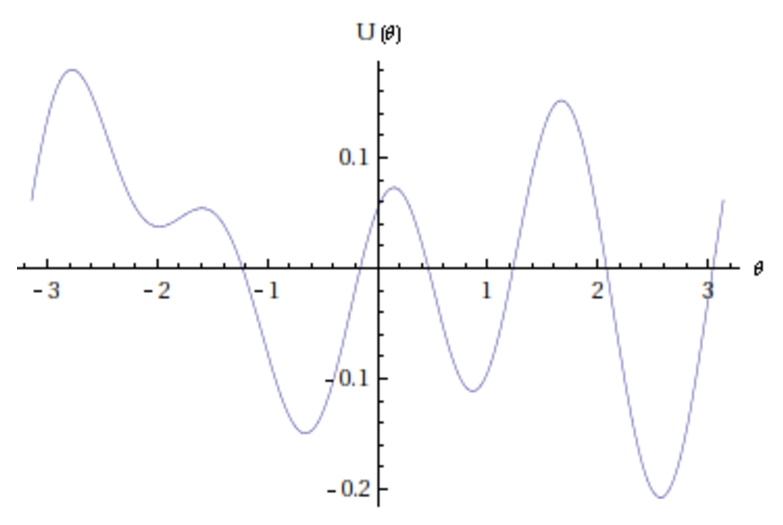
\includegraphics[width=0.45\textwidth]{ks22sliceCond}
 ~~(b)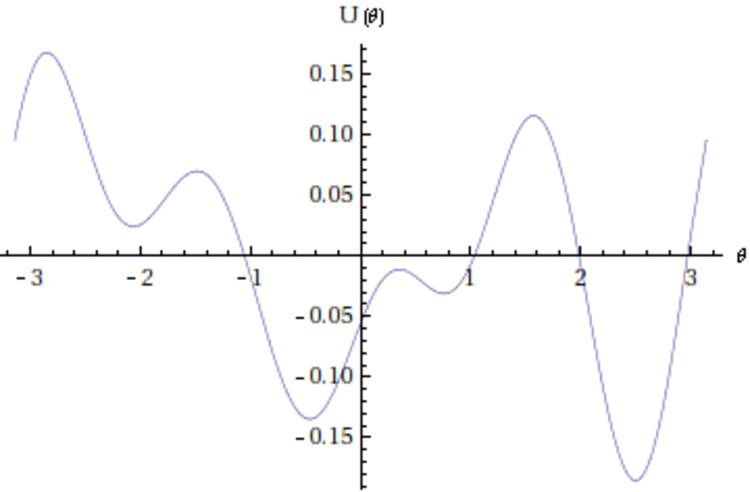
\includegraphics[width=0.45\textwidth]{ks22sliceCond2}
 }{}{
Two snapshots of slice fixing condition \refeq{slicFixTW1} along \rpo\
with $\period{p}=16.31,\shift_p=-2.863$.
}{ks22sliceCond}
%%%%%%%%%%%%%%%%%%%%%%%%%%%%%%%%%%%%%%%%%%%%%%%%%%%%%%%%%%%%%%%%%%%%%


What I find remarkable about \reffigs{ks22rpo16mf}{ks22rposMF} is that
I see no $ \dot{\gSpace} \to \pm\infty$ jumps.

%%%%%%%%%%%%%%%%%%%%%%%%%%%%%%%%%%%%%%%%%%%%%%%%%%%%%%%%%%%%%%%%%%%%%
\FIG{
 (a)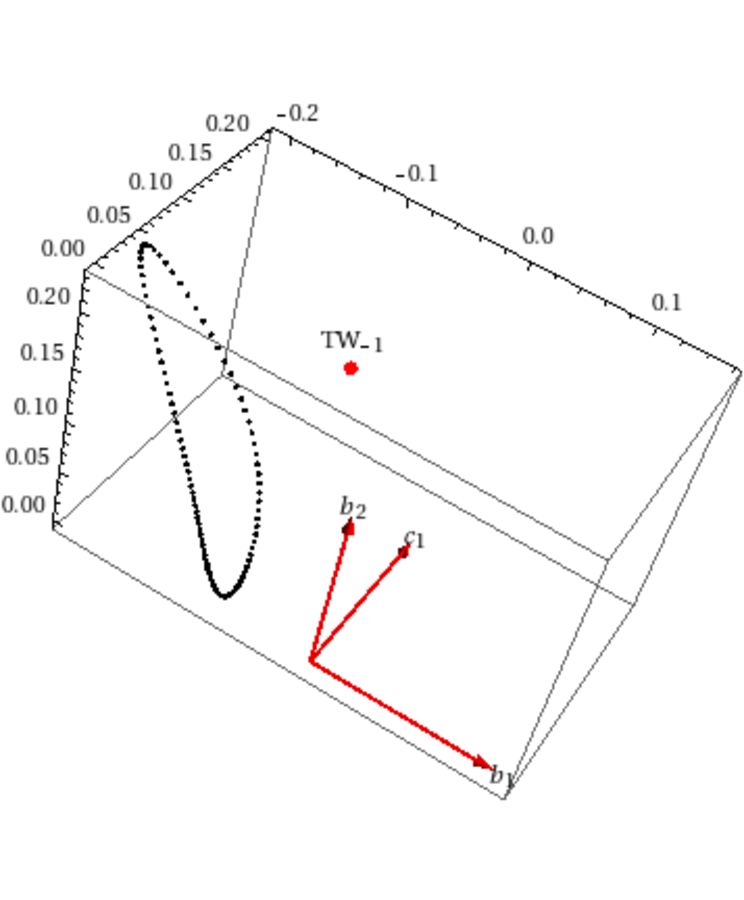
\includegraphics[width=0.45\textwidth]{ks22rpo16mf}
 ~~(b)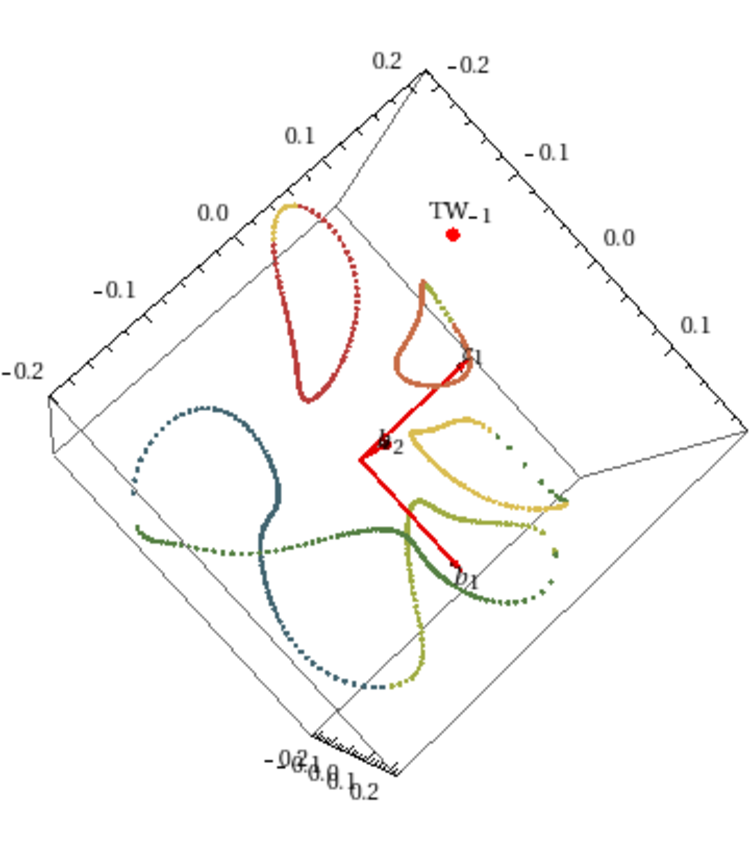
\includegraphics[width=0.45\textwidth]{ks22rpo16mfAll}
 }{}{
\Rpo\ with $\period{p}=16.31,\shift_p=-2.863$ on the \refeq{slicFixTW1} slice.
(a) Tracking solution that corresponds to $\theta$ that maps
$x_p(0)$ to a point of minimum distance from
$\ssp_{TW_{-1}}$,
(b) Accept all $\theta$ and plot all corresponding points.
Color-coding represents internal numbering of solutions and
changes along orbits when the number of solutions for
$\theta$ changes. Note that we have $3$ closed-loop images of
the rpo and $3$ images that appear to connect to a closed
loop. It appears there might be a discrete symmetry here but
I haven't been able to show this.
}{ks22rpo16mf}
%%%%%%%%%%%%%%%%%%%%%%%%%%%%%%%%%%%%%%%%%%%%%%%%%%%%%%%%%%%%%%%%%%%%%

%%%%%%%%%%%%%%%%%%%%%%%%%%%%%%%%%%%%%%%%%%%%%%%%%%%%%%%%%%%%%%%%%%%%%
\FIG{
 (a)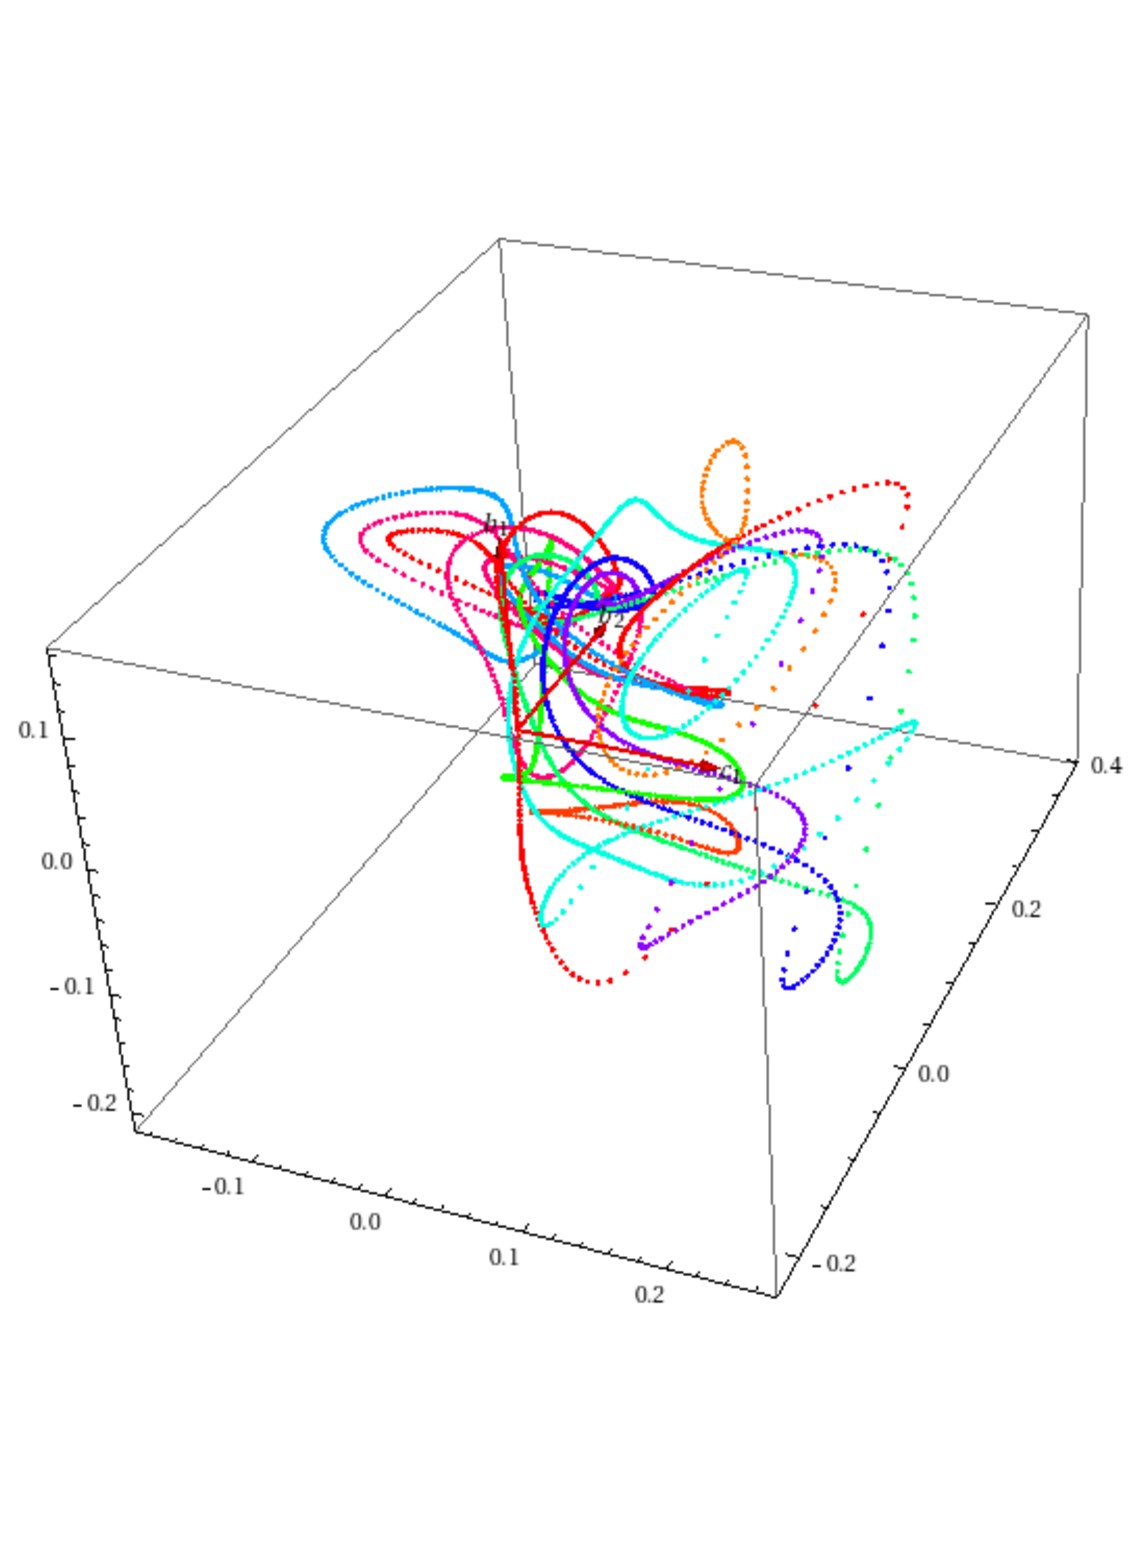
\includegraphics[width=0.45\textwidth]{ks22rposMF}
 ~~(b)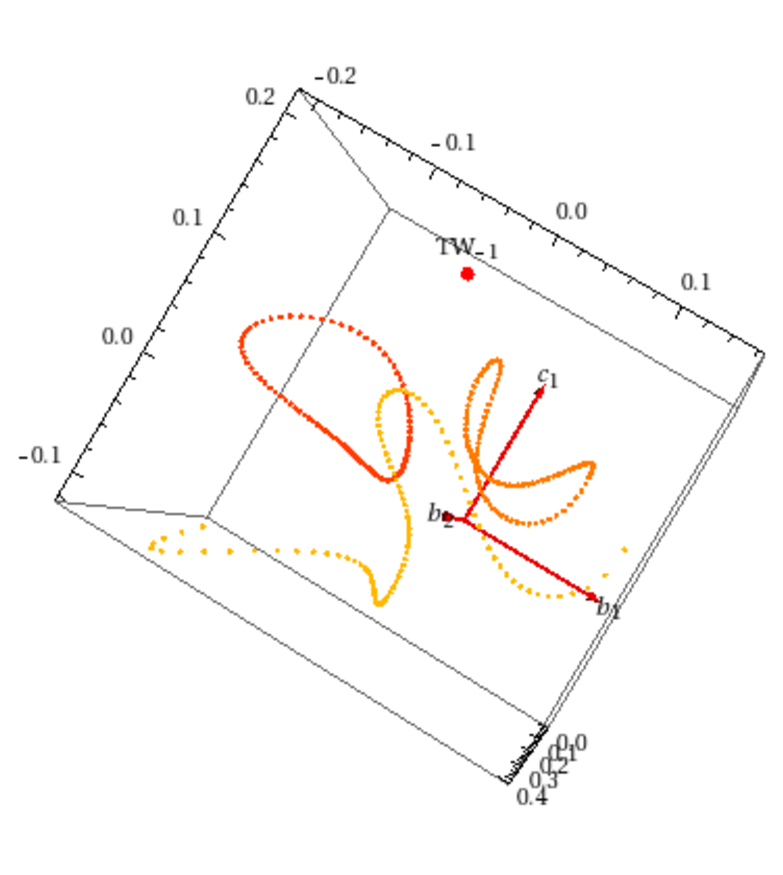
\includegraphics[width=0.45\textwidth]{ks22mf3rpo}
 }{}{
(a) Sample \rpo s and \po s that appear as closed loops after
symmetry reduction through a moving frame that maps them on
on the \refeq{slicFixTW1} slice.
(b)  \Rpo\ with $\period{p}=16.31,\, \shift_p=-2.863$ and \po\ with
$\period{p}=20.51$ appear as closed loops on the slice. \Rpo\ with
$\period{p}=32.80,\, \shift=10.958$ does not appear closed when mapped
back to the slice (the branch that is at minimum distance
from $\ssp_{TW_{-1}}$). We could still have a closed loop
solution but tracking the branches is something I will leave
for later.
}{ks22rposMF}
%%%%%%%%%%%%%%%%%%%%%%%%%%%%%%%%%%%%%%%%%%%%%%%%%%%%%%%%%%%%%%%%%%%%%

\item[2010-01-04 Evangelos]
The good news is that using a traveling wave to
fix a slice was sufficient to reduce about 40\%\ of the short orbits I've
tested to closed loops. For the rest we need a different slice.

\item[2010-01-05 Predrag] Do not understand. Are you saying that the
60\%\ of the short orbits you have tried do not close after one relative period,
or that they encounter the $ \dot{\gSpace} \to \pm\infty$ jumps?

\item[2010-01-05 Evangelos] Sorry, I was not clear on this. 60\%\ of the short orbits
I have tried do not close after one relative period. Since I just use the finite
transformations version (the ``moving frame method'') I do not need to worry about
$ \dot{\gSpace} \to \pm\infty$ jumps. There is some stretching of some orbits even the
ones that are closed loops after reduction, but it is not a great concern.

I wonder whether method of slices (integration on the slice) and moving
frame method (post-processing approach followed
here) fail at the same points. In theory the latter should only fail at points left invariant
under a continuous subgroup, for KS only at the origin. In practice where a moving frame
fails also depends on the choice of slice as we have seen in \cLe.

\item[2010-01-05 Predrag] If the dot product of slice tangent
and orbit tangent are dominated by 3rd Fourier mode, \rpo\
will close only after 3rd repeat, so run them for several
periods.

\Mslices\ and \mframes\ `fail' at the same point, where the
denominator in the reconstruction equation goes through zero.
They do not fail, they just have a $\pi$ jump there.

Why do you guys keep saying that the \mslices\ fails for the
\Fix{\Group}\ flow-invariant subspace? The subspace is within
the slice. $\dot{\gSpace}=0$, the slice velocity equals the
full space velocity, so there is no problem, methinks.

\end{description}

\renewcommand{\LieElrep}{\ensuremath{\mathbf{G}}} % Siminos Lie group element
\renewcommand{\LieEl}{\ensuremath{\gamma}}  % also a Siminos Lie group element
\renewcommand{\gSpace}{\ensuremath{{\bf \theta}}}   % group rotation parameters

\section{2010-01-07 Blogging on}

\begin{description}
\item[2010-01-07 Predrag]
Erik Bollt says that your methods of iteratively refining
symbolic dynamics from periodic orbits might work for KS
orbits. I cannot see how he would do it for RPOs (Euclidean
distance is used), but maybe he can get some symbolic
dynamics from the pre-periodic 20,000 orbits?

\item[2010-01-08 Ruslan]
The problem with this approach is that one has to have a
rough idea of the partition to start with, so it can then be
refined using longer orbits.  It worked well for Henon and
Ikeda, but couldn't cope with more complicated 2-dim maps,
e.g. Ueda attractor, having 5-6 fixed points and needing at
least as many symbols).

A while ago I did some work along similar lines when I looked
at the 'proximity' of chaotic orbits to RPOs.  This piece was
not included in our paper, but it must be floating somewhere
(see, e.g., my talk
/siminos/rpo\_ks/davidchack/GaTech030507.ppt).

This is an empirical approach based essentially on a
combination of pattern recognition and time series analysis:
pieces of orbits that look similar (i.e. are close to each
other in phase space in any appropriate metric) can be
labeled by the same 'symbol'.  Then we can try to construct
a transition matrix between symbols based on the observations
of which patterns follow which.  If we manage to do this for
periodic orbits (both RPOs and PPOs) we may be able to get a
rough idea of the dynamical structure of the system.
There is no problem with symmetries here, since we can define
a metric by minimizing the distance with respect to shift and
reflection.

If what I'm doing now fails, I may get back to this idea.

\item[2010-01-05 Evangelos]
Gr\"obner basis $\neq$ Hilbert basis.

\item[2010-01-07 Predrag] Splitting hairs?:
\HREF{http://en.wikipedia.org/wiki/Hilbert\%27s_basis_theorem}
{en.wikipedia.org/wiki/Hilbert's basis theorem}:
Hilbert method does not give an algorithm
to produce the finitely many basis polynomials for a given
ideal: it only shows that they must exist. One can determine
basis polynomials using the method of Gr\"obner bases.
{\bf ES} Yes, but why not?

\item[2009-12-22 Evangelos]
What do you think about setting up a cns group at zotero:
\HREF{http://www.zotero.org/blog/synchronize-pdfs-and-collaborate-with-zotero/}
{www.zotero.org/blog/synchronize-pdfs-and-collaborate-with-zotero}
  to keep track of important and hard of find papers?

\item[2010-01-07 Predrag] Sounds great, would not mind paying 20 bucks for the
storage. The only thing is - have not found it yet in their FAQs
\begin{enumerate}
   \item access should
be controlled by a group administrator, as materials are copyrighted.
  {\bf ES} My understanding is this is true.
   \item should maintain siminos.bib in the format we have now, the
crap zotero sticks into ziminoz.bib drives me nuts.
  {\bf ES} There is some script that controls export of bib files
      and it is user-tunable. The problem is it might require lots 
      of work -- I have no time for hacking.
\end{enumerate}
Why don't you play with a potential CNS zotero group site for a while,
see how it works? {\bf ES} Will do and blog about it. We have to take care
to organize it in some robust, gibsonian way right at the beginning, though.



\item[2010-01-23 Evangelos]
Using EventLocator testing/flows/CLEfinal.nb I checked that
integration on the slice for CLe approaches but does not
reach singularity.

\item[2010-02-02 Predrag]
The holidays are over. ``That integration on the slice for
CLe approaches but does not reach singularity" worries me. I
would feel better if you checked the crossing by the method
of moving frames, \ie, integrate the full system and keep the
sign relative to the 3-dim subspace. I suspect it crosses,
but if we integrate in the slice the integrator fights against it,
keeps the \reducedsp\ trajectory on one side of the $\infty$- reduced
velocity abyss.

\item[2010-02-03 Evangelos]
Actually I've checked it using moving frames before checking using slices.
I was afraid that in moving frames I just sample points that have the same
sign and miss crossings of the singularity. No, both methods show the same.
One more think I should try is to switch to a more brutal integrator,
see how it behaves. 

The way I see it is that with the general linear slice, together with the
orientation condition we introduce some sort of generalized polar 
radius that cannot become less than zero. In contrast if we do not impose
the orientation condition we really get into trouble: both me and Halcrow
tried that with ZM and I think what we got was real discontinuities in the flow.
Rebecca also had this problem in exercise 2.19 of her blog, where she used
$\cos(\theta)$ to define the moving frame. This is not shown in her figure
2.1, as she only plots her trajectory for $t$ up to $50$. I've proposed to her to
integrate up to $t=200$ and see what happens but she did not do it. What you
will see is a two-eared attractor with instant transitions between ears 
in certain projections. Anyway, this is all post-processing. I do not really
understand why, but in the method of slices orientation condition is satisfied without
us enforcing it. So, what I mean by saying we do not have a problem
with CLE and the method of slices, is not that there is no singularity, but that we stay on
one side of it.

\item[2010-02-03 Evangelos] I will run some more tests but I am kind 
of fed up with CLe, I want to go back to the real thing and try 
to get it to work with KS. 

\end{description}

\section{2010-02-05 ES: Zoteromania}

I've experimentally set up a cns zotero group. 

\begin{tabular}{rl}
 User name 	& cns\\
 pass 		& you don't need it for access\\
 email 		& vaggelis.siminos@gmail.com (temporary)\\
Group name 	& cns\\
group site 	& \HREF{http://www.zotero.org/groups/cns}{http://www.zotero.org/groups/cns} \\
\end{tabular}\\

To subscribe to it you will need a free zotero account, register
\HREF{https://www.zotero.org/user/register/}{here}. Then navigate
to the group \HREF{http://www.zotero.org/groups/cns}{site} and
ask to become member of the group. To sync with the library you 
will need to enable syncing at your zotero firefox plugin preferences.

There are only some test entries in the library right now, we will need
to think a bit about the structure before creating collections. So it's
better not to invite more people to use it right now.

Group access options are:
\begin{description}
 \item[Public, Open Membership] Anyone can view your group online and join the group instantly.
 \item[Public, Closed Membership] Anyone can view your group online, but members must apply or be invited.
 \item[Private Membership] Only members can view your group online and must be invited to join.
\end{description}

ES has chosen Public, Closed Membership. I've also fine tuned the settings so that anyone in the
web can see the database, but only group members can change the database and see attachments, that
is pdf files. We can also restrict the privilege to change entries and files to group admins. This would
prevent accidental loss of data due to someone not knowing what he is doing, but then it won't be
possible for members to easily contribute entries.




\renewcommand{\ssp}{a}
